\documentclass[twoside]{book}

% Packages required by doxygen
\usepackage{fixltx2e}
\usepackage{calc}
\usepackage{doxygen}
\usepackage[export]{adjustbox} % also loads graphicx
\usepackage{graphicx}
\usepackage[utf8]{inputenc}
\usepackage{makeidx}
\usepackage{multicol}
\usepackage{multirow}
\PassOptionsToPackage{warn}{textcomp}
\usepackage{textcomp}
\usepackage[nointegrals]{wasysym}
\usepackage[table]{xcolor}

% Font selection
\usepackage[T1]{fontenc}
\usepackage[scaled=.90]{helvet}
\usepackage{courier}
\usepackage{amssymb}
\usepackage{sectsty}
\renewcommand{\familydefault}{\sfdefault}
\allsectionsfont{%
  \fontseries{bc}\selectfont%
  \color{darkgray}%
}
\renewcommand{\DoxyLabelFont}{%
  \fontseries{bc}\selectfont%
  \color{darkgray}%
}
\newcommand{\+}{\discretionary{\mbox{\scriptsize$\hookleftarrow$}}{}{}}

% Page & text layout
\usepackage{geometry}
\geometry{%
  a4paper,%
  top=2.5cm,%
  bottom=2.5cm,%
  left=2.5cm,%
  right=2.5cm%
}
\tolerance=750
\hfuzz=15pt
\hbadness=750
\setlength{\emergencystretch}{15pt}
\setlength{\parindent}{0cm}
\setlength{\parskip}{3ex plus 2ex minus 2ex}
\makeatletter
\renewcommand{\paragraph}{%
  \@startsection{paragraph}{4}{0ex}{-1.0ex}{1.0ex}{%
    \normalfont\normalsize\bfseries\SS@parafont%
  }%
}
\renewcommand{\subparagraph}{%
  \@startsection{subparagraph}{5}{0ex}{-1.0ex}{1.0ex}{%
    \normalfont\normalsize\bfseries\SS@subparafont%
  }%
}
\makeatother

% Headers & footers
\usepackage{fancyhdr}
\pagestyle{fancyplain}
\fancyhead[LE]{\fancyplain{}{\bfseries\thepage}}
\fancyhead[CE]{\fancyplain{}{}}
\fancyhead[RE]{\fancyplain{}{\bfseries\leftmark}}
\fancyhead[LO]{\fancyplain{}{\bfseries\rightmark}}
\fancyhead[CO]{\fancyplain{}{}}
\fancyhead[RO]{\fancyplain{}{\bfseries\thepage}}
\fancyfoot[LE]{\fancyplain{}{}}
\fancyfoot[CE]{\fancyplain{}{}}
\fancyfoot[RE]{\fancyplain{}{\bfseries\scriptsize Generated by Doxygen }}
\fancyfoot[LO]{\fancyplain{}{\bfseries\scriptsize Generated by Doxygen }}
\fancyfoot[CO]{\fancyplain{}{}}
\fancyfoot[RO]{\fancyplain{}{}}
\renewcommand{\footrulewidth}{0.4pt}
\renewcommand{\chaptermark}[1]{%
  \markboth{#1}{}%
}
\renewcommand{\sectionmark}[1]{%
  \markright{\thesection\ #1}%
}

% Indices & bibliography
\usepackage{natbib}
\usepackage[titles]{tocloft}
\setcounter{tocdepth}{3}
\setcounter{secnumdepth}{5}
\makeindex

% Hyperlinks (required, but should be loaded last)
\usepackage{ifpdf}
\ifpdf
  \usepackage[pdftex,pagebackref=true]{hyperref}
\else
  \usepackage[ps2pdf,pagebackref=true]{hyperref}
\fi
\hypersetup{%
  colorlinks=true,%
  linkcolor=blue,%
  citecolor=blue,%
  unicode%
}

% Custom commands
\newcommand{\clearemptydoublepage}{%
  \newpage{\pagestyle{empty}\cleardoublepage}%
}

\usepackage{caption}
\captionsetup{labelsep=space,justification=centering,font={bf},singlelinecheck=off,skip=4pt,position=top}

%===== C O N T E N T S =====

\begin{document}

% Titlepage & ToC
\hypersetup{pageanchor=false,
             bookmarksnumbered=true,
             pdfencoding=unicode
            }
\pagenumbering{alph}
\begin{titlepage}
\vspace*{7cm}
\begin{center}%
{\Large Pozyx\+Framework }\\
\vspace*{1cm}
{\large Generated by Doxygen 1.8.13}\\
\end{center}
\end{titlepage}
\clearemptydoublepage
\pagenumbering{roman}
\tableofcontents
\clearemptydoublepage
\pagenumbering{arabic}
\hypersetup{pageanchor=true}

%--- Begin generated contents ---
\chapter{Namespace Index}
\section{Packages}
Here are the packages with brief descriptions (if available)\+:\begin{DoxyCompactList}
\item\contentsline{section}{\hyperlink{namespace_pozyx_subscriber}{Pozyx\+Subscriber} }{\pageref{namespace_pozyx_subscriber}}{}
\item\contentsline{section}{\hyperlink{namespace_pozyx_subscriber_1_1_application}{Pozyx\+Subscriber.\+Application} }{\pageref{namespace_pozyx_subscriber_1_1_application}}{}
\item\contentsline{section}{\hyperlink{namespace_pozyx_subscriber_1_1_framework}{Pozyx\+Subscriber.\+Framework} }{\pageref{namespace_pozyx_subscriber_1_1_framework}}{}
\end{DoxyCompactList}

\chapter{Class Index}
\section{Class List}
Here are the classes, structs, unions and interfaces with brief descriptions\+:\begin{DoxyCompactList}
\item\contentsline{section}{\hyperlink{class_pozyx_subscriber_1_1_framework_1_1_anchor}{Pozyx\+Subscriber.\+Framework.\+Anchor} }{\pageref{class_pozyx_subscriber_1_1_framework_1_1_anchor}}{}
\item\contentsline{section}{\hyperlink{class_pozyx_subscriber_1_1_framework_1_1_mqtt_client}{Pozyx\+Subscriber.\+Framework.\+Mqtt\+Client} \\*Mqqt client for subscribing to pozyx broker }{\pageref{class_pozyx_subscriber_1_1_framework_1_1_mqtt_client}}{}
\item\contentsline{section}{\hyperlink{struct_pozyx_subscriber_1_1_framework_1_1_pos_data}{Pozyx\+Subscriber.\+Framework.\+Pos\+Data} \\*Contains a set of position data }{\pageref{struct_pozyx_subscriber_1_1_framework_1_1_pos_data}}{}
\item\contentsline{section}{\hyperlink{struct_pozyx_subscriber_1_1_framework_1_1_pozyx_vector}{Pozyx\+Subscriber.\+Framework.\+Pozyx\+Vector} }{\pageref{struct_pozyx_subscriber_1_1_framework_1_1_pozyx_vector}}{}
\item\contentsline{section}{\hyperlink{class_pozyx_subscriber_1_1_application_1_1_program}{Pozyx\+Subscriber.\+Application.\+Program} }{\pageref{class_pozyx_subscriber_1_1_application_1_1_program}}{}
\item\contentsline{section}{\hyperlink{class_pozyx_subscriber_1_1_framework_1_1_reader}{Pozyx\+Subscriber.\+Framework.\+Reader} \\*Mqqt client for subscribing to pozyx broker }{\pageref{class_pozyx_subscriber_1_1_framework_1_1_reader}}{}
\item\contentsline{section}{\hyperlink{class_pozyx_subscriber_1_1_sim_environment}{Pozyx\+Subscriber.\+Sim\+Environment} \\*Simulation enviornemnt }{\pageref{class_pozyx_subscriber_1_1_sim_environment}}{}
\item\contentsline{section}{\hyperlink{class_pozyx_subscriber_1_1_framework_1_1_sim_object}{Pozyx\+Subscriber.\+Framework.\+Sim\+Object} }{\pageref{class_pozyx_subscriber_1_1_framework_1_1_sim_object}}{}
\item\contentsline{section}{\hyperlink{class_pozyx_subscriber_1_1_framework_1_1_tag}{Pozyx\+Subscriber.\+Framework.\+Tag} }{\pageref{class_pozyx_subscriber_1_1_framework_1_1_tag}}{}
\end{DoxyCompactList}

\chapter{File Index}
\section{File List}
Here is a list of all files with brief descriptions\+:\begin{DoxyCompactList}
\item\contentsline{section}{Project/\+Pozyx\+Subscriber/\+Pozyx\+Subscriber/\hyperlink{_application_8cs}{Application.\+cs} }{\pageref{_application_8cs}}{}
\item\contentsline{section}{Project/\+Pozyx\+Subscriber/\+Pozyx\+Subscriber/\+Application/\hyperlink{_application_2_application_8cs}{Application.\+cs} }{\pageref{_application_2_application_8cs}}{}
\item\contentsline{section}{Project/\+Pozyx\+Subscriber/\+Pozyx\+Subscriber/\+Framework/\hyperlink{_anchor_8cs}{Anchor.\+cs} }{\pageref{_anchor_8cs}}{}
\item\contentsline{section}{Project/\+Pozyx\+Subscriber/\+Pozyx\+Subscriber/\+Framework/\hyperlink{_file_reader_8cs}{File\+Reader.\+cs} }{\pageref{_file_reader_8cs}}{}
\item\contentsline{section}{Project/\+Pozyx\+Subscriber/\+Pozyx\+Subscriber/\+Framework/\hyperlink{_pos_data_8cs}{Pos\+Data.\+cs} }{\pageref{_pos_data_8cs}}{}
\item\contentsline{section}{Project/\+Pozyx\+Subscriber/\+Pozyx\+Subscriber/\+Framework/\hyperlink{_sim_object_8cs}{Sim\+Object.\+cs} }{\pageref{_sim_object_8cs}}{}
\item\contentsline{section}{Project/\+Pozyx\+Subscriber/\+Pozyx\+Subscriber/\+Framework/\hyperlink{_simulation_environment_8cs}{Simulation\+Environment.\+cs} }{\pageref{_simulation_environment_8cs}}{}
\item\contentsline{section}{Project/\+Pozyx\+Subscriber/\+Pozyx\+Subscriber/\+Framework/\hyperlink{_subscriber_8cs}{Subscriber.\+cs} }{\pageref{_subscriber_8cs}}{}
\item\contentsline{section}{Project/\+Pozyx\+Subscriber/\+Pozyx\+Subscriber/\+Framework/\hyperlink{_vector3_d_node_8cs}{Vector3\+D\+Node.\+cs} }{\pageref{_vector3_d_node_8cs}}{}
\item\contentsline{section}{Project/\+Pozyx\+Subscriber/\+Pozyx\+Subscriber/obj/\+Debug/net6.\+0/\hyperlink{_debug_2net6_80_2_8_n_e_t_core_app_00_version_0Av6_80_8_assembly_attributes_8cs}{.\+N\+E\+T\+Core\+App,\+Version=v6.\+0.\+Assembly\+Attributes.\+cs} }{\pageref{_debug_2net6_80_2_8_n_e_t_core_app_00_version_0Av6_80_8_assembly_attributes_8cs}}{}
\item\contentsline{section}{Project/\+Pozyx\+Subscriber/\+Pozyx\+Subscriber/obj/\+Debug/net6.\+0/\hyperlink{_debug_2net6_80_2_pozyx_subscriber_8_assembly_info_8cs}{Pozyx\+Subscriber.\+Assembly\+Info.\+cs} }{\pageref{_debug_2net6_80_2_pozyx_subscriber_8_assembly_info_8cs}}{}
\item\contentsline{section}{Project/\+Pozyx\+Subscriber/\+Pozyx\+Subscriber/obj/\+Debug/net6.\+0/\hyperlink{_debug_2net6_80_2_pozyx_subscriber_8_global_usings_8g_8cs}{Pozyx\+Subscriber.\+Global\+Usings.\+g.\+cs} }{\pageref{_debug_2net6_80_2_pozyx_subscriber_8_global_usings_8g_8cs}}{}
\item\contentsline{section}{Project/\+Pozyx\+Subscriber/\+Pozyx\+Subscriber/obj/\+Debug/net7.\+0/\hyperlink{_8_n_e_t_core_app_00_version_0Av7_80_8_assembly_attributes_8cs}{.\+N\+E\+T\+Core\+App,\+Version=v7.\+0.\+Assembly\+Attributes.\+cs} }{\pageref{_8_n_e_t_core_app_00_version_0Av7_80_8_assembly_attributes_8cs}}{}
\item\contentsline{section}{Project/\+Pozyx\+Subscriber/\+Pozyx\+Subscriber/obj/\+Debug/net7.\+0/\hyperlink{_debug_2net7_80_2_pozyx_subscriber_8_assembly_info_8cs}{Pozyx\+Subscriber.\+Assembly\+Info.\+cs} }{\pageref{_debug_2net7_80_2_pozyx_subscriber_8_assembly_info_8cs}}{}
\item\contentsline{section}{Project/\+Pozyx\+Subscriber/\+Pozyx\+Subscriber/obj/\+Debug/net7.\+0/\hyperlink{_debug_2net7_80_2_pozyx_subscriber_8_global_usings_8g_8cs}{Pozyx\+Subscriber.\+Global\+Usings.\+g.\+cs} }{\pageref{_debug_2net7_80_2_pozyx_subscriber_8_global_usings_8g_8cs}}{}
\item\contentsline{section}{Project/\+Pozyx\+Subscriber/\+Pozyx\+Subscriber/obj/\+Debug/netcoreapp1.\+0/\hyperlink{_8_n_e_t_core_app_00_version_0Av1_80_8_assembly_attributes_8cs}{.\+N\+E\+T\+Core\+App,\+Version=v1.\+0.\+Assembly\+Attributes.\+cs} }{\pageref{_8_n_e_t_core_app_00_version_0Av1_80_8_assembly_attributes_8cs}}{}
\item\contentsline{section}{Project/\+Pozyx\+Subscriber/\+Pozyx\+Subscriber/obj/\+Debug/netcoreapp1.\+0/\hyperlink{_debug_2netcoreapp1_80_2_pozyx_subscriber_8_assembly_info_8cs}{Pozyx\+Subscriber.\+Assembly\+Info.\+cs} }{\pageref{_debug_2netcoreapp1_80_2_pozyx_subscriber_8_assembly_info_8cs}}{}
\item\contentsline{section}{Project/\+Pozyx\+Subscriber/\+Pozyx\+Subscriber/obj/\+Debug/netcoreapp1.\+0/\hyperlink{_debug_2netcoreapp1_80_2_pozyx_subscriber_8_global_usings_8g_8cs}{Pozyx\+Subscriber.\+Global\+Usings.\+g.\+cs} }{\pageref{_debug_2netcoreapp1_80_2_pozyx_subscriber_8_global_usings_8g_8cs}}{}
\item\contentsline{section}{Project/\+Pozyx\+Subscriber/\+Pozyx\+Subscriber/obj/\+Release/net6.\+0/\hyperlink{_release_2net6_80_2_8_n_e_t_core_app_00_version_0Av6_80_8_assembly_attributes_8cs}{.\+N\+E\+T\+Core\+App,\+Version=v6.\+0.\+Assembly\+Attributes.\+cs} }{\pageref{_release_2net6_80_2_8_n_e_t_core_app_00_version_0Av6_80_8_assembly_attributes_8cs}}{}
\item\contentsline{section}{Project/\+Pozyx\+Subscriber/\+Pozyx\+Subscriber/obj/\+Release/net6.\+0/\hyperlink{_release_2net6_80_2_pozyx_subscriber_8_assembly_info_8cs}{Pozyx\+Subscriber.\+Assembly\+Info.\+cs} }{\pageref{_release_2net6_80_2_pozyx_subscriber_8_assembly_info_8cs}}{}
\item\contentsline{section}{Project/\+Pozyx\+Subscriber/\+Pozyx\+Subscriber/obj/\+Release/net6.\+0/\hyperlink{_release_2net6_80_2_pozyx_subscriber_8_global_usings_8g_8cs}{Pozyx\+Subscriber.\+Global\+Usings.\+g.\+cs} }{\pageref{_release_2net6_80_2_pozyx_subscriber_8_global_usings_8g_8cs}}{}
\end{DoxyCompactList}

\chapter{Namespace Documentation}
\hypertarget{namespace_pozyx_subscriber}{}\section{Pozyx\+Subscriber Namespace Reference}
\label{namespace_pozyx_subscriber}\index{Pozyx\+Subscriber@{Pozyx\+Subscriber}}
\subsection*{Namespaces}
\begin{DoxyCompactItemize}
\item 
namespace \hyperlink{namespace_pozyx_subscriber_1_1_application}{Application}
\item 
namespace \hyperlink{namespace_pozyx_subscriber_1_1_framework}{Framework}
\end{DoxyCompactItemize}
\subsection*{Classes}
\begin{DoxyCompactItemize}
\item 
class \hyperlink{class_pozyx_subscriber_1_1_sim_environment}{Sim\+Environment}
\begin{DoxyCompactList}\small\item\em Simulation enviornemnt \end{DoxyCompactList}\end{DoxyCompactItemize}

\hypertarget{namespace_pozyx_subscriber_1_1_application}{}\section{Pozyx\+Subscriber.\+Application Namespace Reference}
\label{namespace_pozyx_subscriber_1_1_application}\index{Pozyx\+Subscriber.\+Application@{Pozyx\+Subscriber.\+Application}}
\subsection*{Classes}
\begin{DoxyCompactItemize}
\item 
class \hyperlink{class_pozyx_subscriber_1_1_application_1_1_program}{Program}
\end{DoxyCompactItemize}

\hypertarget{namespace_pozyx_subscriber_1_1_framework}{}\section{Pozyx\+Subscriber.\+Framework Namespace Reference}
\label{namespace_pozyx_subscriber_1_1_framework}\index{Pozyx\+Subscriber.\+Framework@{Pozyx\+Subscriber.\+Framework}}
\subsection*{Classes}
\begin{DoxyCompactItemize}
\item 
class \hyperlink{class_pozyx_subscriber_1_1_framework_1_1_anchor}{Anchor}
\end{DoxyCompactItemize}

\chapter{Class Documentation}
\hypertarget{class_pozyx_subscriber_1_1_framework_1_1_anchor}{}\section{Pozyx\+Subscriber.\+Framework.\+Anchor Class Reference}
\label{class_pozyx_subscriber_1_1_framework_1_1_anchor}\index{Pozyx\+Subscriber.\+Framework.\+Anchor@{Pozyx\+Subscriber.\+Framework.\+Anchor}}


Collaboration diagram for Pozyx\+Subscriber.\+Framework.\+Anchor\+:
\nopagebreak
\begin{figure}[H]
\begin{center}
\leavevmode
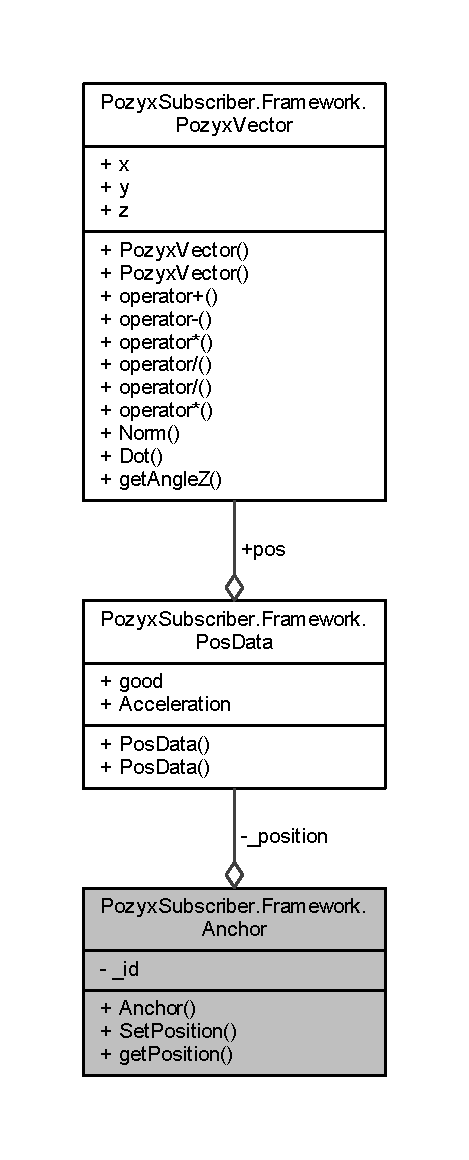
\includegraphics[height=550pt]{class_pozyx_subscriber_1_1_framework_1_1_anchor__coll__graph}
\end{center}
\end{figure}
\subsection*{Public Member Functions}
\begin{DoxyCompactItemize}
\item 
\hyperlink{class_pozyx_subscriber_1_1_framework_1_1_anchor_af3383b1c654f08e99fd5fd42a522b1b7}{Anchor} (string ID)
\item 
void \hyperlink{class_pozyx_subscriber_1_1_framework_1_1_anchor_a7a7f74dc8d89d8ec6bbd5f155fce5850}{Set\+Position} (float x, float y, float z)
\item 
\hyperlink{struct_pozyx_subscriber_1_1_framework_1_1_pos_data}{Pos\+Data} \hyperlink{class_pozyx_subscriber_1_1_framework_1_1_anchor_aa62fb67e660b0a83467bca1e8a523607}{get\+Position} ()
\end{DoxyCompactItemize}
\subsection*{Private Attributes}
\begin{DoxyCompactItemize}
\item 
\hyperlink{struct_pozyx_subscriber_1_1_framework_1_1_pos_data}{Pos\+Data} \hyperlink{class_pozyx_subscriber_1_1_framework_1_1_anchor_ac316ecc8136e9a3081a847c41854e67a}{\+\_\+position}
\item 
string \hyperlink{class_pozyx_subscriber_1_1_framework_1_1_anchor_a2bd63c7b8f0f8d466e6e4da6a1d89cab}{\+\_\+id}
\end{DoxyCompactItemize}


\subsection{Constructor \& Destructor Documentation}
\mbox{\Hypertarget{class_pozyx_subscriber_1_1_framework_1_1_anchor_af3383b1c654f08e99fd5fd42a522b1b7}\label{class_pozyx_subscriber_1_1_framework_1_1_anchor_af3383b1c654f08e99fd5fd42a522b1b7}} 
\index{Pozyx\+Subscriber\+::\+Framework\+::\+Anchor@{Pozyx\+Subscriber\+::\+Framework\+::\+Anchor}!Anchor@{Anchor}}
\index{Anchor@{Anchor}!Pozyx\+Subscriber\+::\+Framework\+::\+Anchor@{Pozyx\+Subscriber\+::\+Framework\+::\+Anchor}}
\subsubsection{\texorpdfstring{Anchor()}{Anchor()}}
{\footnotesize\ttfamily Pozyx\+Subscriber.\+Framework.\+Anchor.\+Anchor (\begin{DoxyParamCaption}\item[{string}]{ID }\end{DoxyParamCaption})}



\subsection{Member Function Documentation}
\mbox{\Hypertarget{class_pozyx_subscriber_1_1_framework_1_1_anchor_aa62fb67e660b0a83467bca1e8a523607}\label{class_pozyx_subscriber_1_1_framework_1_1_anchor_aa62fb67e660b0a83467bca1e8a523607}} 
\index{Pozyx\+Subscriber\+::\+Framework\+::\+Anchor@{Pozyx\+Subscriber\+::\+Framework\+::\+Anchor}!get\+Position@{get\+Position}}
\index{get\+Position@{get\+Position}!Pozyx\+Subscriber\+::\+Framework\+::\+Anchor@{Pozyx\+Subscriber\+::\+Framework\+::\+Anchor}}
\subsubsection{\texorpdfstring{get\+Position()}{getPosition()}}
{\footnotesize\ttfamily \hyperlink{struct_pozyx_subscriber_1_1_framework_1_1_pos_data}{Pos\+Data} Pozyx\+Subscriber.\+Framework.\+Anchor.\+get\+Position (\begin{DoxyParamCaption}{ }\end{DoxyParamCaption})}

\mbox{\Hypertarget{class_pozyx_subscriber_1_1_framework_1_1_anchor_a7a7f74dc8d89d8ec6bbd5f155fce5850}\label{class_pozyx_subscriber_1_1_framework_1_1_anchor_a7a7f74dc8d89d8ec6bbd5f155fce5850}} 
\index{Pozyx\+Subscriber\+::\+Framework\+::\+Anchor@{Pozyx\+Subscriber\+::\+Framework\+::\+Anchor}!Set\+Position@{Set\+Position}}
\index{Set\+Position@{Set\+Position}!Pozyx\+Subscriber\+::\+Framework\+::\+Anchor@{Pozyx\+Subscriber\+::\+Framework\+::\+Anchor}}
\subsubsection{\texorpdfstring{Set\+Position()}{SetPosition()}}
{\footnotesize\ttfamily void Pozyx\+Subscriber.\+Framework.\+Anchor.\+Set\+Position (\begin{DoxyParamCaption}\item[{float}]{x,  }\item[{float}]{y,  }\item[{float}]{z }\end{DoxyParamCaption})}



\subsection{Member Data Documentation}
\mbox{\Hypertarget{class_pozyx_subscriber_1_1_framework_1_1_anchor_a2bd63c7b8f0f8d466e6e4da6a1d89cab}\label{class_pozyx_subscriber_1_1_framework_1_1_anchor_a2bd63c7b8f0f8d466e6e4da6a1d89cab}} 
\index{Pozyx\+Subscriber\+::\+Framework\+::\+Anchor@{Pozyx\+Subscriber\+::\+Framework\+::\+Anchor}!\+\_\+id@{\+\_\+id}}
\index{\+\_\+id@{\+\_\+id}!Pozyx\+Subscriber\+::\+Framework\+::\+Anchor@{Pozyx\+Subscriber\+::\+Framework\+::\+Anchor}}
\subsubsection{\texorpdfstring{\+\_\+id}{\_id}}
{\footnotesize\ttfamily string Pozyx\+Subscriber.\+Framework.\+Anchor.\+\_\+id\hspace{0.3cm}{\ttfamily [private]}}

\mbox{\Hypertarget{class_pozyx_subscriber_1_1_framework_1_1_anchor_ac316ecc8136e9a3081a847c41854e67a}\label{class_pozyx_subscriber_1_1_framework_1_1_anchor_ac316ecc8136e9a3081a847c41854e67a}} 
\index{Pozyx\+Subscriber\+::\+Framework\+::\+Anchor@{Pozyx\+Subscriber\+::\+Framework\+::\+Anchor}!\+\_\+position@{\+\_\+position}}
\index{\+\_\+position@{\+\_\+position}!Pozyx\+Subscriber\+::\+Framework\+::\+Anchor@{Pozyx\+Subscriber\+::\+Framework\+::\+Anchor}}
\subsubsection{\texorpdfstring{\+\_\+position}{\_position}}
{\footnotesize\ttfamily \hyperlink{struct_pozyx_subscriber_1_1_framework_1_1_pos_data}{Pos\+Data} Pozyx\+Subscriber.\+Framework.\+Anchor.\+\_\+position\hspace{0.3cm}{\ttfamily [private]}}



The documentation for this class was generated from the following file\+:\begin{DoxyCompactItemize}
\item 
Project/\+Pozyx\+Subscriber/\+Pozyx\+Subscriber/\+Framework/\hyperlink{_anchor_8cs}{Anchor.\+cs}\end{DoxyCompactItemize}

\hypertarget{class_pozyx_subscriber_1_1_framework_1_1_mqtt_client}{}\section{Pozyx\+Subscriber.\+Framework.\+Mqtt\+Client Class Reference}
\label{class_pozyx_subscriber_1_1_framework_1_1_mqtt_client}\index{Pozyx\+Subscriber.\+Framework.\+Mqtt\+Client@{Pozyx\+Subscriber.\+Framework.\+Mqtt\+Client}}


Mqqt client for subscribing to pozyx broker  




Collaboration diagram for Pozyx\+Subscriber.\+Framework.\+Mqtt\+Client\+:
\nopagebreak
\begin{figure}[H]
\begin{center}
\leavevmode
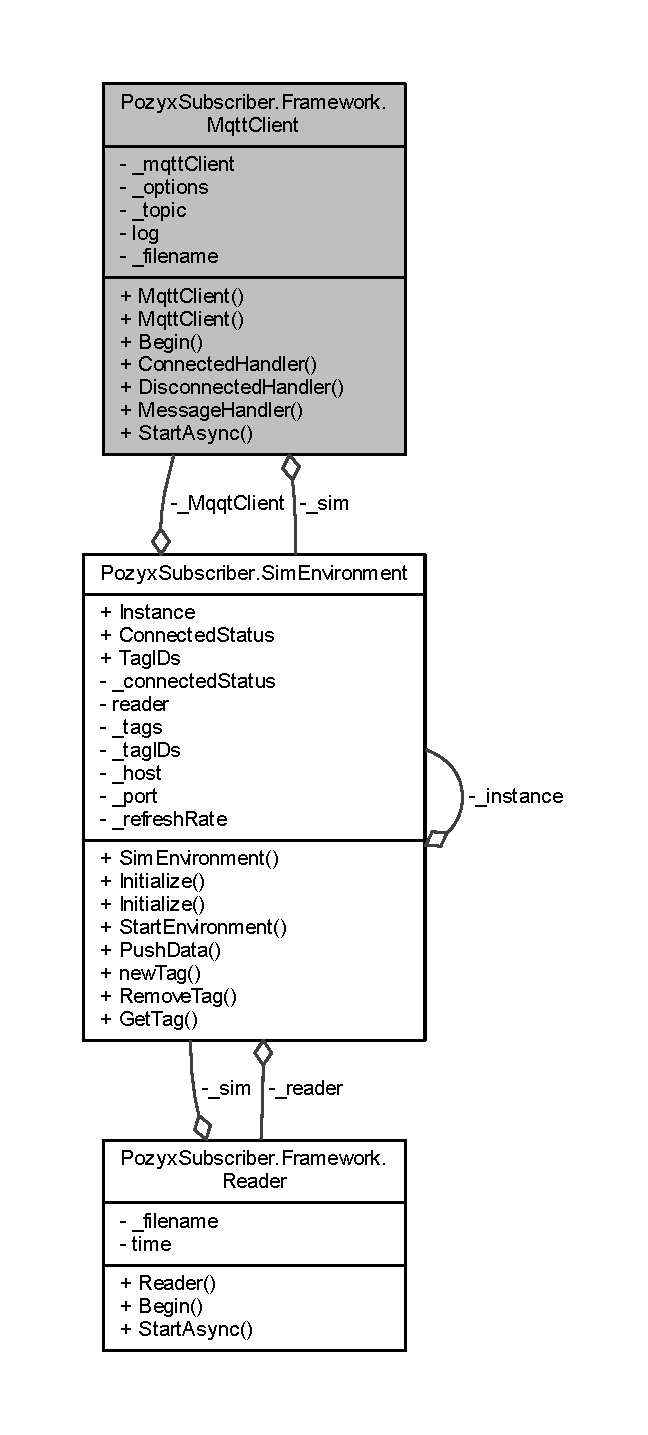
\includegraphics[height=550pt]{class_pozyx_subscriber_1_1_framework_1_1_mqtt_client__coll__graph}
\end{center}
\end{figure}
\subsection*{Public Member Functions}
\begin{DoxyCompactItemize}
\item 
\hyperlink{class_pozyx_subscriber_1_1_framework_1_1_mqtt_client_ad2d247e2046c2a43f823e77a94802545}{Mqtt\+Client} (string host, int port, \hyperlink{class_pozyx_subscriber_1_1_sim_environment}{Sim\+Environment} Sim)
\begin{DoxyCompactList}\small\item\em Initializes and begins asynch subscription to tag topic from pozyx broker \end{DoxyCompactList}\item 
\hyperlink{class_pozyx_subscriber_1_1_framework_1_1_mqtt_client_aeeb12e63278f50106a6d5fb6605d2f0b}{Mqtt\+Client} (string host, int port, \hyperlink{class_pozyx_subscriber_1_1_sim_environment}{Sim\+Environment} Sim, string filename)
\item 
void \hyperlink{class_pozyx_subscriber_1_1_framework_1_1_mqtt_client_aab2a4adc47c58e9de1e307d0c8f467dc}{Begin} ()
\item 
async void \hyperlink{class_pozyx_subscriber_1_1_framework_1_1_mqtt_client_a88bca5e01f7b0aa1279d0b92cff3b03b}{Connected\+Handler} (Mqtt\+Client\+Connected\+Event\+Args e)
\item 
void \hyperlink{class_pozyx_subscriber_1_1_framework_1_1_mqtt_client_acabf34348d05e247155adf10d7632b6f}{Disconnected\+Handler} (Mqtt\+Client\+Disconnected\+Event\+Args event\+Args)
\item 
void \hyperlink{class_pozyx_subscriber_1_1_framework_1_1_mqtt_client_a5ee71b80d7ae09ef3a487a5762094b7e}{Message\+Handler} (Mqtt\+Application\+Message\+Received\+Event\+Args event\+Args)
\item 
async Task \hyperlink{class_pozyx_subscriber_1_1_framework_1_1_mqtt_client_a0fc53bbaeb9efec6fa5d8ad5708e3fae}{Start\+Async} ()
\end{DoxyCompactItemize}
\subsection*{Private Attributes}
\begin{DoxyCompactItemize}
\item 
I\+Mqtt\+Client \hyperlink{class_pozyx_subscriber_1_1_framework_1_1_mqtt_client_a87eef1b4acc1a34131cba51200b1d769}{\+\_\+mqtt\+Client}
\item 
I\+Mqtt\+Client\+Options \hyperlink{class_pozyx_subscriber_1_1_framework_1_1_mqtt_client_a02914fcd8ac56b10a6cd5c29a4a6b64e}{\+\_\+options}
\item 
string \hyperlink{class_pozyx_subscriber_1_1_framework_1_1_mqtt_client_a87701d3f45a0c6149f9a7305144713f8}{\+\_\+topic}
\item 
\hyperlink{class_pozyx_subscriber_1_1_sim_environment}{Sim\+Environment} \hyperlink{class_pozyx_subscriber_1_1_framework_1_1_mqtt_client_ab65cd6844648eb75a68ffe881f80beea}{\+\_\+sim}
\item 
String\+Builder \hyperlink{class_pozyx_subscriber_1_1_framework_1_1_mqtt_client_a5ed77cbca2ee86d73a18d0dedb1bbe99}{log} = new String\+Builder()
\item 
string \hyperlink{class_pozyx_subscriber_1_1_framework_1_1_mqtt_client_ae52e36480c57296f8c88230dac699a95}{\+\_\+filename}
\end{DoxyCompactItemize}


\subsection{Detailed Description}
Mqqt client for subscribing to pozyx broker 



\subsection{Constructor \& Destructor Documentation}
\mbox{\Hypertarget{class_pozyx_subscriber_1_1_framework_1_1_mqtt_client_ad2d247e2046c2a43f823e77a94802545}\label{class_pozyx_subscriber_1_1_framework_1_1_mqtt_client_ad2d247e2046c2a43f823e77a94802545}} 
\index{Pozyx\+Subscriber\+::\+Framework\+::\+Mqtt\+Client@{Pozyx\+Subscriber\+::\+Framework\+::\+Mqtt\+Client}!Mqtt\+Client@{Mqtt\+Client}}
\index{Mqtt\+Client@{Mqtt\+Client}!Pozyx\+Subscriber\+::\+Framework\+::\+Mqtt\+Client@{Pozyx\+Subscriber\+::\+Framework\+::\+Mqtt\+Client}}
\subsubsection{\texorpdfstring{Mqtt\+Client()}{MqttClient()}\hspace{0.1cm}{\footnotesize\ttfamily [1/2]}}
{\footnotesize\ttfamily Pozyx\+Subscriber.\+Framework.\+Mqtt\+Client.\+Mqtt\+Client (\begin{DoxyParamCaption}\item[{string}]{host,  }\item[{int}]{port,  }\item[{\hyperlink{class_pozyx_subscriber_1_1_sim_environment}{Sim\+Environment}}]{Sim }\end{DoxyParamCaption})}



Initializes and begins asynch subscription to tag topic from pozyx broker 


\begin{DoxyParams}{Parameters}
{\em \+\_\+num\+Tags} & Number of tags to be tracked\\
\hline
{\em host} & Host of the pozyx broker\\
\hline
{\em port} & Port\\
\hline
\end{DoxyParams}
\mbox{\Hypertarget{class_pozyx_subscriber_1_1_framework_1_1_mqtt_client_aeeb12e63278f50106a6d5fb6605d2f0b}\label{class_pozyx_subscriber_1_1_framework_1_1_mqtt_client_aeeb12e63278f50106a6d5fb6605d2f0b}} 
\index{Pozyx\+Subscriber\+::\+Framework\+::\+Mqtt\+Client@{Pozyx\+Subscriber\+::\+Framework\+::\+Mqtt\+Client}!Mqtt\+Client@{Mqtt\+Client}}
\index{Mqtt\+Client@{Mqtt\+Client}!Pozyx\+Subscriber\+::\+Framework\+::\+Mqtt\+Client@{Pozyx\+Subscriber\+::\+Framework\+::\+Mqtt\+Client}}
\subsubsection{\texorpdfstring{Mqtt\+Client()}{MqttClient()}\hspace{0.1cm}{\footnotesize\ttfamily [2/2]}}
{\footnotesize\ttfamily Pozyx\+Subscriber.\+Framework.\+Mqtt\+Client.\+Mqtt\+Client (\begin{DoxyParamCaption}\item[{string}]{host,  }\item[{int}]{port,  }\item[{\hyperlink{class_pozyx_subscriber_1_1_sim_environment}{Sim\+Environment}}]{Sim,  }\item[{string}]{filename }\end{DoxyParamCaption})}



\subsection{Member Function Documentation}
\mbox{\Hypertarget{class_pozyx_subscriber_1_1_framework_1_1_mqtt_client_aab2a4adc47c58e9de1e307d0c8f467dc}\label{class_pozyx_subscriber_1_1_framework_1_1_mqtt_client_aab2a4adc47c58e9de1e307d0c8f467dc}} 
\index{Pozyx\+Subscriber\+::\+Framework\+::\+Mqtt\+Client@{Pozyx\+Subscriber\+::\+Framework\+::\+Mqtt\+Client}!Begin@{Begin}}
\index{Begin@{Begin}!Pozyx\+Subscriber\+::\+Framework\+::\+Mqtt\+Client@{Pozyx\+Subscriber\+::\+Framework\+::\+Mqtt\+Client}}
\subsubsection{\texorpdfstring{Begin()}{Begin()}}
{\footnotesize\ttfamily void Pozyx\+Subscriber.\+Framework.\+Mqtt\+Client.\+Begin (\begin{DoxyParamCaption}{ }\end{DoxyParamCaption})}

Here is the caller graph for this function\+:
\nopagebreak
\begin{figure}[H]
\begin{center}
\leavevmode
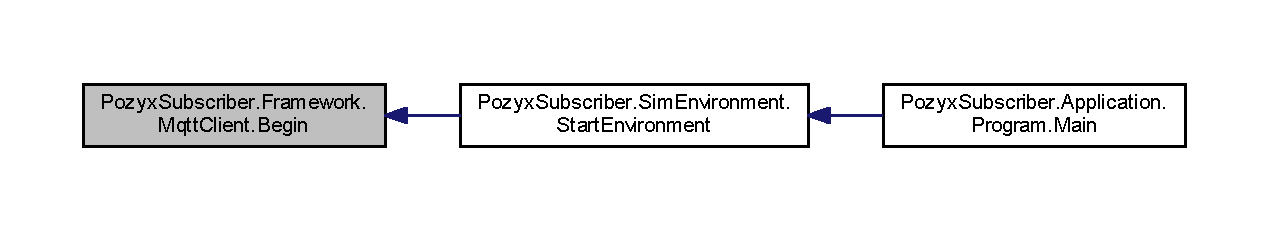
\includegraphics[width=350pt]{class_pozyx_subscriber_1_1_framework_1_1_mqtt_client_aab2a4adc47c58e9de1e307d0c8f467dc_icgraph}
\end{center}
\end{figure}
\mbox{\Hypertarget{class_pozyx_subscriber_1_1_framework_1_1_mqtt_client_a88bca5e01f7b0aa1279d0b92cff3b03b}\label{class_pozyx_subscriber_1_1_framework_1_1_mqtt_client_a88bca5e01f7b0aa1279d0b92cff3b03b}} 
\index{Pozyx\+Subscriber\+::\+Framework\+::\+Mqtt\+Client@{Pozyx\+Subscriber\+::\+Framework\+::\+Mqtt\+Client}!Connected\+Handler@{Connected\+Handler}}
\index{Connected\+Handler@{Connected\+Handler}!Pozyx\+Subscriber\+::\+Framework\+::\+Mqtt\+Client@{Pozyx\+Subscriber\+::\+Framework\+::\+Mqtt\+Client}}
\subsubsection{\texorpdfstring{Connected\+Handler()}{ConnectedHandler()}}
{\footnotesize\ttfamily async void Pozyx\+Subscriber.\+Framework.\+Mqtt\+Client.\+Connected\+Handler (\begin{DoxyParamCaption}\item[{Mqtt\+Client\+Connected\+Event\+Args}]{e }\end{DoxyParamCaption})}

\mbox{\Hypertarget{class_pozyx_subscriber_1_1_framework_1_1_mqtt_client_acabf34348d05e247155adf10d7632b6f}\label{class_pozyx_subscriber_1_1_framework_1_1_mqtt_client_acabf34348d05e247155adf10d7632b6f}} 
\index{Pozyx\+Subscriber\+::\+Framework\+::\+Mqtt\+Client@{Pozyx\+Subscriber\+::\+Framework\+::\+Mqtt\+Client}!Disconnected\+Handler@{Disconnected\+Handler}}
\index{Disconnected\+Handler@{Disconnected\+Handler}!Pozyx\+Subscriber\+::\+Framework\+::\+Mqtt\+Client@{Pozyx\+Subscriber\+::\+Framework\+::\+Mqtt\+Client}}
\subsubsection{\texorpdfstring{Disconnected\+Handler()}{DisconnectedHandler()}}
{\footnotesize\ttfamily void Pozyx\+Subscriber.\+Framework.\+Mqtt\+Client.\+Disconnected\+Handler (\begin{DoxyParamCaption}\item[{Mqtt\+Client\+Disconnected\+Event\+Args}]{event\+Args }\end{DoxyParamCaption})}

\mbox{\Hypertarget{class_pozyx_subscriber_1_1_framework_1_1_mqtt_client_a5ee71b80d7ae09ef3a487a5762094b7e}\label{class_pozyx_subscriber_1_1_framework_1_1_mqtt_client_a5ee71b80d7ae09ef3a487a5762094b7e}} 
\index{Pozyx\+Subscriber\+::\+Framework\+::\+Mqtt\+Client@{Pozyx\+Subscriber\+::\+Framework\+::\+Mqtt\+Client}!Message\+Handler@{Message\+Handler}}
\index{Message\+Handler@{Message\+Handler}!Pozyx\+Subscriber\+::\+Framework\+::\+Mqtt\+Client@{Pozyx\+Subscriber\+::\+Framework\+::\+Mqtt\+Client}}
\subsubsection{\texorpdfstring{Message\+Handler()}{MessageHandler()}}
{\footnotesize\ttfamily void Pozyx\+Subscriber.\+Framework.\+Mqtt\+Client.\+Message\+Handler (\begin{DoxyParamCaption}\item[{Mqtt\+Application\+Message\+Received\+Event\+Args}]{event\+Args }\end{DoxyParamCaption})}

Here is the call graph for this function\+:
\nopagebreak
\begin{figure}[H]
\begin{center}
\leavevmode
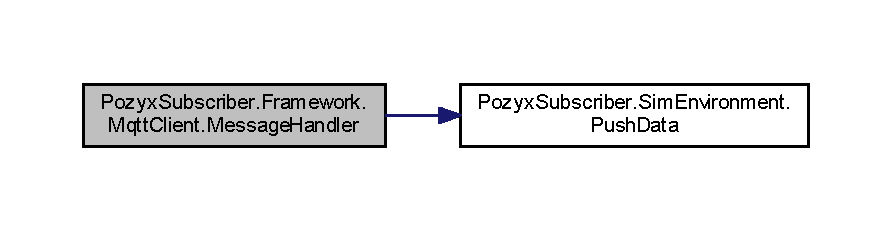
\includegraphics[width=350pt]{class_pozyx_subscriber_1_1_framework_1_1_mqtt_client_a5ee71b80d7ae09ef3a487a5762094b7e_cgraph}
\end{center}
\end{figure}
\mbox{\Hypertarget{class_pozyx_subscriber_1_1_framework_1_1_mqtt_client_a0fc53bbaeb9efec6fa5d8ad5708e3fae}\label{class_pozyx_subscriber_1_1_framework_1_1_mqtt_client_a0fc53bbaeb9efec6fa5d8ad5708e3fae}} 
\index{Pozyx\+Subscriber\+::\+Framework\+::\+Mqtt\+Client@{Pozyx\+Subscriber\+::\+Framework\+::\+Mqtt\+Client}!Start\+Async@{Start\+Async}}
\index{Start\+Async@{Start\+Async}!Pozyx\+Subscriber\+::\+Framework\+::\+Mqtt\+Client@{Pozyx\+Subscriber\+::\+Framework\+::\+Mqtt\+Client}}
\subsubsection{\texorpdfstring{Start\+Async()}{StartAsync()}}
{\footnotesize\ttfamily async Task Pozyx\+Subscriber.\+Framework.\+Mqtt\+Client.\+Start\+Async (\begin{DoxyParamCaption}{ }\end{DoxyParamCaption})}



\subsection{Member Data Documentation}
\mbox{\Hypertarget{class_pozyx_subscriber_1_1_framework_1_1_mqtt_client_ae52e36480c57296f8c88230dac699a95}\label{class_pozyx_subscriber_1_1_framework_1_1_mqtt_client_ae52e36480c57296f8c88230dac699a95}} 
\index{Pozyx\+Subscriber\+::\+Framework\+::\+Mqtt\+Client@{Pozyx\+Subscriber\+::\+Framework\+::\+Mqtt\+Client}!\+\_\+filename@{\+\_\+filename}}
\index{\+\_\+filename@{\+\_\+filename}!Pozyx\+Subscriber\+::\+Framework\+::\+Mqtt\+Client@{Pozyx\+Subscriber\+::\+Framework\+::\+Mqtt\+Client}}
\subsubsection{\texorpdfstring{\+\_\+filename}{\_filename}}
{\footnotesize\ttfamily string Pozyx\+Subscriber.\+Framework.\+Mqtt\+Client.\+\_\+filename\hspace{0.3cm}{\ttfamily [private]}}

\mbox{\Hypertarget{class_pozyx_subscriber_1_1_framework_1_1_mqtt_client_a87eef1b4acc1a34131cba51200b1d769}\label{class_pozyx_subscriber_1_1_framework_1_1_mqtt_client_a87eef1b4acc1a34131cba51200b1d769}} 
\index{Pozyx\+Subscriber\+::\+Framework\+::\+Mqtt\+Client@{Pozyx\+Subscriber\+::\+Framework\+::\+Mqtt\+Client}!\+\_\+mqtt\+Client@{\+\_\+mqtt\+Client}}
\index{\+\_\+mqtt\+Client@{\+\_\+mqtt\+Client}!Pozyx\+Subscriber\+::\+Framework\+::\+Mqtt\+Client@{Pozyx\+Subscriber\+::\+Framework\+::\+Mqtt\+Client}}
\subsubsection{\texorpdfstring{\+\_\+mqtt\+Client}{\_mqttClient}}
{\footnotesize\ttfamily I\+Mqtt\+Client Pozyx\+Subscriber.\+Framework.\+Mqtt\+Client.\+\_\+mqtt\+Client\hspace{0.3cm}{\ttfamily [private]}}

\mbox{\Hypertarget{class_pozyx_subscriber_1_1_framework_1_1_mqtt_client_a02914fcd8ac56b10a6cd5c29a4a6b64e}\label{class_pozyx_subscriber_1_1_framework_1_1_mqtt_client_a02914fcd8ac56b10a6cd5c29a4a6b64e}} 
\index{Pozyx\+Subscriber\+::\+Framework\+::\+Mqtt\+Client@{Pozyx\+Subscriber\+::\+Framework\+::\+Mqtt\+Client}!\+\_\+options@{\+\_\+options}}
\index{\+\_\+options@{\+\_\+options}!Pozyx\+Subscriber\+::\+Framework\+::\+Mqtt\+Client@{Pozyx\+Subscriber\+::\+Framework\+::\+Mqtt\+Client}}
\subsubsection{\texorpdfstring{\+\_\+options}{\_options}}
{\footnotesize\ttfamily I\+Mqtt\+Client\+Options Pozyx\+Subscriber.\+Framework.\+Mqtt\+Client.\+\_\+options\hspace{0.3cm}{\ttfamily [private]}}

\mbox{\Hypertarget{class_pozyx_subscriber_1_1_framework_1_1_mqtt_client_ab65cd6844648eb75a68ffe881f80beea}\label{class_pozyx_subscriber_1_1_framework_1_1_mqtt_client_ab65cd6844648eb75a68ffe881f80beea}} 
\index{Pozyx\+Subscriber\+::\+Framework\+::\+Mqtt\+Client@{Pozyx\+Subscriber\+::\+Framework\+::\+Mqtt\+Client}!\+\_\+sim@{\+\_\+sim}}
\index{\+\_\+sim@{\+\_\+sim}!Pozyx\+Subscriber\+::\+Framework\+::\+Mqtt\+Client@{Pozyx\+Subscriber\+::\+Framework\+::\+Mqtt\+Client}}
\subsubsection{\texorpdfstring{\+\_\+sim}{\_sim}}
{\footnotesize\ttfamily \hyperlink{class_pozyx_subscriber_1_1_sim_environment}{Sim\+Environment} Pozyx\+Subscriber.\+Framework.\+Mqtt\+Client.\+\_\+sim\hspace{0.3cm}{\ttfamily [private]}}

\mbox{\Hypertarget{class_pozyx_subscriber_1_1_framework_1_1_mqtt_client_a87701d3f45a0c6149f9a7305144713f8}\label{class_pozyx_subscriber_1_1_framework_1_1_mqtt_client_a87701d3f45a0c6149f9a7305144713f8}} 
\index{Pozyx\+Subscriber\+::\+Framework\+::\+Mqtt\+Client@{Pozyx\+Subscriber\+::\+Framework\+::\+Mqtt\+Client}!\+\_\+topic@{\+\_\+topic}}
\index{\+\_\+topic@{\+\_\+topic}!Pozyx\+Subscriber\+::\+Framework\+::\+Mqtt\+Client@{Pozyx\+Subscriber\+::\+Framework\+::\+Mqtt\+Client}}
\subsubsection{\texorpdfstring{\+\_\+topic}{\_topic}}
{\footnotesize\ttfamily string Pozyx\+Subscriber.\+Framework.\+Mqtt\+Client.\+\_\+topic\hspace{0.3cm}{\ttfamily [private]}}

\mbox{\Hypertarget{class_pozyx_subscriber_1_1_framework_1_1_mqtt_client_a5ed77cbca2ee86d73a18d0dedb1bbe99}\label{class_pozyx_subscriber_1_1_framework_1_1_mqtt_client_a5ed77cbca2ee86d73a18d0dedb1bbe99}} 
\index{Pozyx\+Subscriber\+::\+Framework\+::\+Mqtt\+Client@{Pozyx\+Subscriber\+::\+Framework\+::\+Mqtt\+Client}!log@{log}}
\index{log@{log}!Pozyx\+Subscriber\+::\+Framework\+::\+Mqtt\+Client@{Pozyx\+Subscriber\+::\+Framework\+::\+Mqtt\+Client}}
\subsubsection{\texorpdfstring{log}{log}}
{\footnotesize\ttfamily String\+Builder Pozyx\+Subscriber.\+Framework.\+Mqtt\+Client.\+log = new String\+Builder()\hspace{0.3cm}{\ttfamily [private]}}



The documentation for this class was generated from the following file\+:\begin{DoxyCompactItemize}
\item 
Project/\+Pozyx\+Subscriber/\+Pozyx\+Subscriber/\+Framework/\hyperlink{_subscriber_8cs}{Subscriber.\+cs}\end{DoxyCompactItemize}

\hypertarget{struct_pozyx_subscriber_1_1_framework_1_1_pos_data}{}\section{Pozyx\+Subscriber.\+Framework.\+Pos\+Data Struct Reference}
\label{struct_pozyx_subscriber_1_1_framework_1_1_pos_data}\index{Pozyx\+Subscriber.\+Framework.\+Pos\+Data@{Pozyx\+Subscriber.\+Framework.\+Pos\+Data}}


Contains a set of position data  




Collaboration diagram for Pozyx\+Subscriber.\+Framework.\+Pos\+Data\+:
% FIG 0
\subsection*{Public Member Functions}
\begin{DoxyCompactItemize}
\item 
\hyperlink{struct_pozyx_subscriber_1_1_framework_1_1_pos_data_aece72e84d2c40a52bba235cdd84d525e}{Pos\+Data} (float \+\_\+x, float \+\_\+y, float \+\_\+z)
\begin{DoxyCompactList}\small\item\em Create position data node with x, y, z coordinates \end{DoxyCompactList}\item 
\hyperlink{struct_pozyx_subscriber_1_1_framework_1_1_pos_data_a11f7d5411a5edea66123a4ba2187705e}{Pos\+Data} ()
\end{DoxyCompactItemize}
\subsection*{Public Attributes}
\begin{DoxyCompactItemize}
\item 
\hyperlink{struct_pozyx_subscriber_1_1_framework_1_1_pozyx_vector}{Pozyx\+Vector} \hyperlink{struct_pozyx_subscriber_1_1_framework_1_1_pos_data_aff147d1e93133ef61c532f5b16ce2d4c}{pos}
\item 
bool \hyperlink{struct_pozyx_subscriber_1_1_framework_1_1_pos_data_adc23be06f8e926708bfca77144f549e6}{good}
\item 
List$<$ \hyperlink{struct_pozyx_subscriber_1_1_framework_1_1_pozyx_vector}{Pozyx\+Vector} $>$ \hyperlink{struct_pozyx_subscriber_1_1_framework_1_1_pos_data_a3a392d3d0fb95980c5fbf152de894370}{Acceleration}
\end{DoxyCompactItemize}


\subsection{Detailed Description}
Contains a set of position data 



\subsection{Constructor \& Destructor Documentation}
\mbox{\Hypertarget{struct_pozyx_subscriber_1_1_framework_1_1_pos_data_aece72e84d2c40a52bba235cdd84d525e}\label{struct_pozyx_subscriber_1_1_framework_1_1_pos_data_aece72e84d2c40a52bba235cdd84d525e}} 
\index{Pozyx\+Subscriber\+::\+Framework\+::\+Pos\+Data@{Pozyx\+Subscriber\+::\+Framework\+::\+Pos\+Data}!Pos\+Data@{Pos\+Data}}
\index{Pos\+Data@{Pos\+Data}!Pozyx\+Subscriber\+::\+Framework\+::\+Pos\+Data@{Pozyx\+Subscriber\+::\+Framework\+::\+Pos\+Data}}
\subsubsection{\texorpdfstring{Pos\+Data()}{PosData()}\hspace{0.1cm}{\footnotesize\ttfamily [1/2]}}
{\footnotesize\ttfamily Pozyx\+Subscriber.\+Framework.\+Pos\+Data.\+Pos\+Data (\begin{DoxyParamCaption}\item[{float}]{\+\_\+x,  }\item[{float}]{\+\_\+y,  }\item[{float}]{\+\_\+z }\end{DoxyParamCaption})}



Create position data node with x, y, z coordinates 


\begin{DoxyParams}{Parameters}
{\em \+\_\+x} & \\
\hline
{\em \+\_\+y} & \\
\hline
{\em \+\_\+z} & \\
\hline
\end{DoxyParams}
\mbox{\Hypertarget{struct_pozyx_subscriber_1_1_framework_1_1_pos_data_a11f7d5411a5edea66123a4ba2187705e}\label{struct_pozyx_subscriber_1_1_framework_1_1_pos_data_a11f7d5411a5edea66123a4ba2187705e}} 
\index{Pozyx\+Subscriber\+::\+Framework\+::\+Pos\+Data@{Pozyx\+Subscriber\+::\+Framework\+::\+Pos\+Data}!Pos\+Data@{Pos\+Data}}
\index{Pos\+Data@{Pos\+Data}!Pozyx\+Subscriber\+::\+Framework\+::\+Pos\+Data@{Pozyx\+Subscriber\+::\+Framework\+::\+Pos\+Data}}
\subsubsection{\texorpdfstring{Pos\+Data()}{PosData()}\hspace{0.1cm}{\footnotesize\ttfamily [2/2]}}
{\footnotesize\ttfamily Pozyx\+Subscriber.\+Framework.\+Pos\+Data.\+Pos\+Data (\begin{DoxyParamCaption}{ }\end{DoxyParamCaption})}



\subsection{Member Data Documentation}
\mbox{\Hypertarget{struct_pozyx_subscriber_1_1_framework_1_1_pos_data_a3a392d3d0fb95980c5fbf152de894370}\label{struct_pozyx_subscriber_1_1_framework_1_1_pos_data_a3a392d3d0fb95980c5fbf152de894370}} 
\index{Pozyx\+Subscriber\+::\+Framework\+::\+Pos\+Data@{Pozyx\+Subscriber\+::\+Framework\+::\+Pos\+Data}!Acceleration@{Acceleration}}
\index{Acceleration@{Acceleration}!Pozyx\+Subscriber\+::\+Framework\+::\+Pos\+Data@{Pozyx\+Subscriber\+::\+Framework\+::\+Pos\+Data}}
\subsubsection{\texorpdfstring{Acceleration}{Acceleration}}
{\footnotesize\ttfamily List$<$\hyperlink{struct_pozyx_subscriber_1_1_framework_1_1_pozyx_vector}{Pozyx\+Vector}$>$ Pozyx\+Subscriber.\+Framework.\+Pos\+Data.\+Acceleration}

\mbox{\Hypertarget{struct_pozyx_subscriber_1_1_framework_1_1_pos_data_adc23be06f8e926708bfca77144f549e6}\label{struct_pozyx_subscriber_1_1_framework_1_1_pos_data_adc23be06f8e926708bfca77144f549e6}} 
\index{Pozyx\+Subscriber\+::\+Framework\+::\+Pos\+Data@{Pozyx\+Subscriber\+::\+Framework\+::\+Pos\+Data}!good@{good}}
\index{good@{good}!Pozyx\+Subscriber\+::\+Framework\+::\+Pos\+Data@{Pozyx\+Subscriber\+::\+Framework\+::\+Pos\+Data}}
\subsubsection{\texorpdfstring{good}{good}}
{\footnotesize\ttfamily bool Pozyx\+Subscriber.\+Framework.\+Pos\+Data.\+good}

\mbox{\Hypertarget{struct_pozyx_subscriber_1_1_framework_1_1_pos_data_aff147d1e93133ef61c532f5b16ce2d4c}\label{struct_pozyx_subscriber_1_1_framework_1_1_pos_data_aff147d1e93133ef61c532f5b16ce2d4c}} 
\index{Pozyx\+Subscriber\+::\+Framework\+::\+Pos\+Data@{Pozyx\+Subscriber\+::\+Framework\+::\+Pos\+Data}!pos@{pos}}
\index{pos@{pos}!Pozyx\+Subscriber\+::\+Framework\+::\+Pos\+Data@{Pozyx\+Subscriber\+::\+Framework\+::\+Pos\+Data}}
\subsubsection{\texorpdfstring{pos}{pos}}
{\footnotesize\ttfamily \hyperlink{struct_pozyx_subscriber_1_1_framework_1_1_pozyx_vector}{Pozyx\+Vector} Pozyx\+Subscriber.\+Framework.\+Pos\+Data.\+pos}



The documentation for this struct was generated from the following file\+:\begin{DoxyCompactItemize}
\item 
Project/\+Pozyx\+Subscriber/\+Pozyx\+Subscriber/\+Framework/\hyperlink{_pos_data_8cs}{Pos\+Data.\+cs}\end{DoxyCompactItemize}

\hypertarget{struct_pozyx_subscriber_1_1_framework_1_1_pozyx_vector}{}\section{Pozyx\+Subscriber.\+Framework.\+Pozyx\+Vector Struct Reference}
\label{struct_pozyx_subscriber_1_1_framework_1_1_pozyx_vector}\index{Pozyx\+Subscriber.\+Framework.\+Pozyx\+Vector@{Pozyx\+Subscriber.\+Framework.\+Pozyx\+Vector}}


Collaboration diagram for Pozyx\+Subscriber.\+Framework.\+Pozyx\+Vector\+:
% FIG 0
\subsection*{Public Member Functions}
\begin{DoxyCompactItemize}
\item 
\hyperlink{struct_pozyx_subscriber_1_1_framework_1_1_pozyx_vector_a9b698d9e83339b4a71856aefdca5e1b6}{Pozyx\+Vector} ()
\item 
\hyperlink{struct_pozyx_subscriber_1_1_framework_1_1_pozyx_vector_ab572bd4a48efe90311b899b86f73fadf}{Pozyx\+Vector} (float \+\_\+x, float \+\_\+y, float \+\_\+z)
\end{DoxyCompactItemize}
\subsection*{Static Public Member Functions}
\begin{DoxyCompactItemize}
\item 
static \hyperlink{struct_pozyx_subscriber_1_1_framework_1_1_pozyx_vector}{Pozyx\+Vector} \hyperlink{struct_pozyx_subscriber_1_1_framework_1_1_pozyx_vector_ad9217e4f7c748ebbcd005656bbb15c07}{operator+} (\hyperlink{struct_pozyx_subscriber_1_1_framework_1_1_pozyx_vector}{Pozyx\+Vector} a, \hyperlink{struct_pozyx_subscriber_1_1_framework_1_1_pozyx_vector}{Pozyx\+Vector} b)
\item 
static \hyperlink{struct_pozyx_subscriber_1_1_framework_1_1_pozyx_vector}{Pozyx\+Vector} \hyperlink{struct_pozyx_subscriber_1_1_framework_1_1_pozyx_vector_ae607f892a7eab44b2385884df61f6699}{operator-\/} (\hyperlink{struct_pozyx_subscriber_1_1_framework_1_1_pozyx_vector}{Pozyx\+Vector} a, \hyperlink{struct_pozyx_subscriber_1_1_framework_1_1_pozyx_vector}{Pozyx\+Vector} b)
\item 
static \hyperlink{struct_pozyx_subscriber_1_1_framework_1_1_pozyx_vector}{Pozyx\+Vector} \hyperlink{struct_pozyx_subscriber_1_1_framework_1_1_pozyx_vector_a46b777f59a80586112c74ff13c27dacc}{operator$\ast$} (\hyperlink{struct_pozyx_subscriber_1_1_framework_1_1_pozyx_vector}{Pozyx\+Vector} a, \hyperlink{struct_pozyx_subscriber_1_1_framework_1_1_pozyx_vector}{Pozyx\+Vector} b)
\item 
static \hyperlink{struct_pozyx_subscriber_1_1_framework_1_1_pozyx_vector}{Pozyx\+Vector} \hyperlink{struct_pozyx_subscriber_1_1_framework_1_1_pozyx_vector_a8319e66719bd50e33a1742a846b2947e}{operator/} (\hyperlink{struct_pozyx_subscriber_1_1_framework_1_1_pozyx_vector}{Pozyx\+Vector} a, \hyperlink{struct_pozyx_subscriber_1_1_framework_1_1_pozyx_vector}{Pozyx\+Vector} b)
\item 
static \hyperlink{struct_pozyx_subscriber_1_1_framework_1_1_pozyx_vector}{Pozyx\+Vector} \hyperlink{struct_pozyx_subscriber_1_1_framework_1_1_pozyx_vector_a68df6b4b698e4a585d613bb7b5763a26}{operator/} (\hyperlink{struct_pozyx_subscriber_1_1_framework_1_1_pozyx_vector}{Pozyx\+Vector} a, float b)
\item 
static \hyperlink{struct_pozyx_subscriber_1_1_framework_1_1_pozyx_vector}{Pozyx\+Vector} \hyperlink{struct_pozyx_subscriber_1_1_framework_1_1_pozyx_vector_ab1b621d997bd4ec029ddec8869b6248e}{operator$\ast$} (\hyperlink{struct_pozyx_subscriber_1_1_framework_1_1_pozyx_vector}{Pozyx\+Vector} a, float b)
\item 
static float \hyperlink{struct_pozyx_subscriber_1_1_framework_1_1_pozyx_vector_a44da2728624c5997efe7a086d1c11356}{Norm} (\hyperlink{struct_pozyx_subscriber_1_1_framework_1_1_pozyx_vector}{Pozyx\+Vector} a)
\item 
static float \hyperlink{struct_pozyx_subscriber_1_1_framework_1_1_pozyx_vector_abc07da4b47b1141e447f0a6a57fbb5fb}{Dot} (\hyperlink{struct_pozyx_subscriber_1_1_framework_1_1_pozyx_vector}{Pozyx\+Vector} a, \hyperlink{struct_pozyx_subscriber_1_1_framework_1_1_pozyx_vector}{Pozyx\+Vector} b)
\item 
static \hyperlink{struct_pozyx_subscriber_1_1_framework_1_1_pozyx_vector}{Pozyx\+Vector} \hyperlink{struct_pozyx_subscriber_1_1_framework_1_1_pozyx_vector_a57884d6f0b0e0ae9d5745ce88848597d}{get\+AngleZ} (\hyperlink{struct_pozyx_subscriber_1_1_framework_1_1_pozyx_vector}{Pozyx\+Vector} a, \hyperlink{struct_pozyx_subscriber_1_1_framework_1_1_pozyx_vector}{Pozyx\+Vector} b)
\end{DoxyCompactItemize}
\subsection*{Public Attributes}
\begin{DoxyCompactItemize}
\item 
float \hyperlink{struct_pozyx_subscriber_1_1_framework_1_1_pozyx_vector_aaf687bd5085dd3c3f7898837f01c83d7}{x}
\item 
float \hyperlink{struct_pozyx_subscriber_1_1_framework_1_1_pozyx_vector_a797da3992cbe6488a25af4dcf7acf297}{y}
\item 
float \hyperlink{struct_pozyx_subscriber_1_1_framework_1_1_pozyx_vector_a600da165d6704d619340ce23e4920b0e}{z}
\end{DoxyCompactItemize}


\subsection{Constructor \& Destructor Documentation}
\mbox{\Hypertarget{struct_pozyx_subscriber_1_1_framework_1_1_pozyx_vector_a9b698d9e83339b4a71856aefdca5e1b6}\label{struct_pozyx_subscriber_1_1_framework_1_1_pozyx_vector_a9b698d9e83339b4a71856aefdca5e1b6}} 
\index{Pozyx\+Subscriber\+::\+Framework\+::\+Pozyx\+Vector@{Pozyx\+Subscriber\+::\+Framework\+::\+Pozyx\+Vector}!Pozyx\+Vector@{Pozyx\+Vector}}
\index{Pozyx\+Vector@{Pozyx\+Vector}!Pozyx\+Subscriber\+::\+Framework\+::\+Pozyx\+Vector@{Pozyx\+Subscriber\+::\+Framework\+::\+Pozyx\+Vector}}
\subsubsection{\texorpdfstring{Pozyx\+Vector()}{PozyxVector()}\hspace{0.1cm}{\footnotesize\ttfamily [1/2]}}
{\footnotesize\ttfamily Pozyx\+Subscriber.\+Framework.\+Pozyx\+Vector.\+Pozyx\+Vector (\begin{DoxyParamCaption}{ }\end{DoxyParamCaption})}

\mbox{\Hypertarget{struct_pozyx_subscriber_1_1_framework_1_1_pozyx_vector_ab572bd4a48efe90311b899b86f73fadf}\label{struct_pozyx_subscriber_1_1_framework_1_1_pozyx_vector_ab572bd4a48efe90311b899b86f73fadf}} 
\index{Pozyx\+Subscriber\+::\+Framework\+::\+Pozyx\+Vector@{Pozyx\+Subscriber\+::\+Framework\+::\+Pozyx\+Vector}!Pozyx\+Vector@{Pozyx\+Vector}}
\index{Pozyx\+Vector@{Pozyx\+Vector}!Pozyx\+Subscriber\+::\+Framework\+::\+Pozyx\+Vector@{Pozyx\+Subscriber\+::\+Framework\+::\+Pozyx\+Vector}}
\subsubsection{\texorpdfstring{Pozyx\+Vector()}{PozyxVector()}\hspace{0.1cm}{\footnotesize\ttfamily [2/2]}}
{\footnotesize\ttfamily Pozyx\+Subscriber.\+Framework.\+Pozyx\+Vector.\+Pozyx\+Vector (\begin{DoxyParamCaption}\item[{float}]{\+\_\+x,  }\item[{float}]{\+\_\+y,  }\item[{float}]{\+\_\+z }\end{DoxyParamCaption})}



\subsection{Member Function Documentation}
\mbox{\Hypertarget{struct_pozyx_subscriber_1_1_framework_1_1_pozyx_vector_abc07da4b47b1141e447f0a6a57fbb5fb}\label{struct_pozyx_subscriber_1_1_framework_1_1_pozyx_vector_abc07da4b47b1141e447f0a6a57fbb5fb}} 
\index{Pozyx\+Subscriber\+::\+Framework\+::\+Pozyx\+Vector@{Pozyx\+Subscriber\+::\+Framework\+::\+Pozyx\+Vector}!Dot@{Dot}}
\index{Dot@{Dot}!Pozyx\+Subscriber\+::\+Framework\+::\+Pozyx\+Vector@{Pozyx\+Subscriber\+::\+Framework\+::\+Pozyx\+Vector}}
\subsubsection{\texorpdfstring{Dot()}{Dot()}}
{\footnotesize\ttfamily static float Pozyx\+Subscriber.\+Framework.\+Pozyx\+Vector.\+Dot (\begin{DoxyParamCaption}\item[{\hyperlink{struct_pozyx_subscriber_1_1_framework_1_1_pozyx_vector}{Pozyx\+Vector}}]{a,  }\item[{\hyperlink{struct_pozyx_subscriber_1_1_framework_1_1_pozyx_vector}{Pozyx\+Vector}}]{b }\end{DoxyParamCaption})\hspace{0.3cm}{\ttfamily [static]}}

\mbox{\Hypertarget{struct_pozyx_subscriber_1_1_framework_1_1_pozyx_vector_a57884d6f0b0e0ae9d5745ce88848597d}\label{struct_pozyx_subscriber_1_1_framework_1_1_pozyx_vector_a57884d6f0b0e0ae9d5745ce88848597d}} 
\index{Pozyx\+Subscriber\+::\+Framework\+::\+Pozyx\+Vector@{Pozyx\+Subscriber\+::\+Framework\+::\+Pozyx\+Vector}!get\+AngleZ@{get\+AngleZ}}
\index{get\+AngleZ@{get\+AngleZ}!Pozyx\+Subscriber\+::\+Framework\+::\+Pozyx\+Vector@{Pozyx\+Subscriber\+::\+Framework\+::\+Pozyx\+Vector}}
\subsubsection{\texorpdfstring{get\+Angle\+Z()}{getAngleZ()}}
{\footnotesize\ttfamily static \hyperlink{struct_pozyx_subscriber_1_1_framework_1_1_pozyx_vector}{Pozyx\+Vector} Pozyx\+Subscriber.\+Framework.\+Pozyx\+Vector.\+get\+AngleZ (\begin{DoxyParamCaption}\item[{\hyperlink{struct_pozyx_subscriber_1_1_framework_1_1_pozyx_vector}{Pozyx\+Vector}}]{a,  }\item[{\hyperlink{struct_pozyx_subscriber_1_1_framework_1_1_pozyx_vector}{Pozyx\+Vector}}]{b }\end{DoxyParamCaption})\hspace{0.3cm}{\ttfamily [static]}}

Here is the caller graph for this function\+:
% FIG 1
\mbox{\Hypertarget{struct_pozyx_subscriber_1_1_framework_1_1_pozyx_vector_a44da2728624c5997efe7a086d1c11356}\label{struct_pozyx_subscriber_1_1_framework_1_1_pozyx_vector_a44da2728624c5997efe7a086d1c11356}} 
\index{Pozyx\+Subscriber\+::\+Framework\+::\+Pozyx\+Vector@{Pozyx\+Subscriber\+::\+Framework\+::\+Pozyx\+Vector}!Norm@{Norm}}
\index{Norm@{Norm}!Pozyx\+Subscriber\+::\+Framework\+::\+Pozyx\+Vector@{Pozyx\+Subscriber\+::\+Framework\+::\+Pozyx\+Vector}}
\subsubsection{\texorpdfstring{Norm()}{Norm()}}
{\footnotesize\ttfamily static float Pozyx\+Subscriber.\+Framework.\+Pozyx\+Vector.\+Norm (\begin{DoxyParamCaption}\item[{\hyperlink{struct_pozyx_subscriber_1_1_framework_1_1_pozyx_vector}{Pozyx\+Vector}}]{a }\end{DoxyParamCaption})\hspace{0.3cm}{\ttfamily [static]}}

\mbox{\Hypertarget{struct_pozyx_subscriber_1_1_framework_1_1_pozyx_vector_a46b777f59a80586112c74ff13c27dacc}\label{struct_pozyx_subscriber_1_1_framework_1_1_pozyx_vector_a46b777f59a80586112c74ff13c27dacc}} 
\index{Pozyx\+Subscriber\+::\+Framework\+::\+Pozyx\+Vector@{Pozyx\+Subscriber\+::\+Framework\+::\+Pozyx\+Vector}!operator$\ast$@{operator$\ast$}}
\index{operator$\ast$@{operator$\ast$}!Pozyx\+Subscriber\+::\+Framework\+::\+Pozyx\+Vector@{Pozyx\+Subscriber\+::\+Framework\+::\+Pozyx\+Vector}}
\subsubsection{\texorpdfstring{operator$\ast$()}{operator*()}\hspace{0.1cm}{\footnotesize\ttfamily [1/2]}}
{\footnotesize\ttfamily static \hyperlink{struct_pozyx_subscriber_1_1_framework_1_1_pozyx_vector}{Pozyx\+Vector} Pozyx\+Subscriber.\+Framework.\+Pozyx\+Vector.\+operator$\ast$ (\begin{DoxyParamCaption}\item[{\hyperlink{struct_pozyx_subscriber_1_1_framework_1_1_pozyx_vector}{Pozyx\+Vector}}]{a,  }\item[{\hyperlink{struct_pozyx_subscriber_1_1_framework_1_1_pozyx_vector}{Pozyx\+Vector}}]{b }\end{DoxyParamCaption})\hspace{0.3cm}{\ttfamily [static]}}

\mbox{\Hypertarget{struct_pozyx_subscriber_1_1_framework_1_1_pozyx_vector_ab1b621d997bd4ec029ddec8869b6248e}\label{struct_pozyx_subscriber_1_1_framework_1_1_pozyx_vector_ab1b621d997bd4ec029ddec8869b6248e}} 
\index{Pozyx\+Subscriber\+::\+Framework\+::\+Pozyx\+Vector@{Pozyx\+Subscriber\+::\+Framework\+::\+Pozyx\+Vector}!operator$\ast$@{operator$\ast$}}
\index{operator$\ast$@{operator$\ast$}!Pozyx\+Subscriber\+::\+Framework\+::\+Pozyx\+Vector@{Pozyx\+Subscriber\+::\+Framework\+::\+Pozyx\+Vector}}
\subsubsection{\texorpdfstring{operator$\ast$()}{operator*()}\hspace{0.1cm}{\footnotesize\ttfamily [2/2]}}
{\footnotesize\ttfamily static \hyperlink{struct_pozyx_subscriber_1_1_framework_1_1_pozyx_vector}{Pozyx\+Vector} Pozyx\+Subscriber.\+Framework.\+Pozyx\+Vector.\+operator$\ast$ (\begin{DoxyParamCaption}\item[{\hyperlink{struct_pozyx_subscriber_1_1_framework_1_1_pozyx_vector}{Pozyx\+Vector}}]{a,  }\item[{float}]{b }\end{DoxyParamCaption})\hspace{0.3cm}{\ttfamily [static]}}

\mbox{\Hypertarget{struct_pozyx_subscriber_1_1_framework_1_1_pozyx_vector_ad9217e4f7c748ebbcd005656bbb15c07}\label{struct_pozyx_subscriber_1_1_framework_1_1_pozyx_vector_ad9217e4f7c748ebbcd005656bbb15c07}} 
\index{Pozyx\+Subscriber\+::\+Framework\+::\+Pozyx\+Vector@{Pozyx\+Subscriber\+::\+Framework\+::\+Pozyx\+Vector}!operator+@{operator+}}
\index{operator+@{operator+}!Pozyx\+Subscriber\+::\+Framework\+::\+Pozyx\+Vector@{Pozyx\+Subscriber\+::\+Framework\+::\+Pozyx\+Vector}}
\subsubsection{\texorpdfstring{operator+()}{operator+()}}
{\footnotesize\ttfamily static \hyperlink{struct_pozyx_subscriber_1_1_framework_1_1_pozyx_vector}{Pozyx\+Vector} Pozyx\+Subscriber.\+Framework.\+Pozyx\+Vector.\+operator+ (\begin{DoxyParamCaption}\item[{\hyperlink{struct_pozyx_subscriber_1_1_framework_1_1_pozyx_vector}{Pozyx\+Vector}}]{a,  }\item[{\hyperlink{struct_pozyx_subscriber_1_1_framework_1_1_pozyx_vector}{Pozyx\+Vector}}]{b }\end{DoxyParamCaption})\hspace{0.3cm}{\ttfamily [static]}}

\mbox{\Hypertarget{struct_pozyx_subscriber_1_1_framework_1_1_pozyx_vector_ae607f892a7eab44b2385884df61f6699}\label{struct_pozyx_subscriber_1_1_framework_1_1_pozyx_vector_ae607f892a7eab44b2385884df61f6699}} 
\index{Pozyx\+Subscriber\+::\+Framework\+::\+Pozyx\+Vector@{Pozyx\+Subscriber\+::\+Framework\+::\+Pozyx\+Vector}!operator-\/@{operator-\/}}
\index{operator-\/@{operator-\/}!Pozyx\+Subscriber\+::\+Framework\+::\+Pozyx\+Vector@{Pozyx\+Subscriber\+::\+Framework\+::\+Pozyx\+Vector}}
\subsubsection{\texorpdfstring{operator-\/()}{operator-()}}
{\footnotesize\ttfamily static \hyperlink{struct_pozyx_subscriber_1_1_framework_1_1_pozyx_vector}{Pozyx\+Vector} Pozyx\+Subscriber.\+Framework.\+Pozyx\+Vector.\+operator-\/ (\begin{DoxyParamCaption}\item[{\hyperlink{struct_pozyx_subscriber_1_1_framework_1_1_pozyx_vector}{Pozyx\+Vector}}]{a,  }\item[{\hyperlink{struct_pozyx_subscriber_1_1_framework_1_1_pozyx_vector}{Pozyx\+Vector}}]{b }\end{DoxyParamCaption})\hspace{0.3cm}{\ttfamily [static]}}

\mbox{\Hypertarget{struct_pozyx_subscriber_1_1_framework_1_1_pozyx_vector_a8319e66719bd50e33a1742a846b2947e}\label{struct_pozyx_subscriber_1_1_framework_1_1_pozyx_vector_a8319e66719bd50e33a1742a846b2947e}} 
\index{Pozyx\+Subscriber\+::\+Framework\+::\+Pozyx\+Vector@{Pozyx\+Subscriber\+::\+Framework\+::\+Pozyx\+Vector}!operator/@{operator/}}
\index{operator/@{operator/}!Pozyx\+Subscriber\+::\+Framework\+::\+Pozyx\+Vector@{Pozyx\+Subscriber\+::\+Framework\+::\+Pozyx\+Vector}}
\subsubsection{\texorpdfstring{operator/()}{operator/()}\hspace{0.1cm}{\footnotesize\ttfamily [1/2]}}
{\footnotesize\ttfamily static \hyperlink{struct_pozyx_subscriber_1_1_framework_1_1_pozyx_vector}{Pozyx\+Vector} Pozyx\+Subscriber.\+Framework.\+Pozyx\+Vector.\+operator/ (\begin{DoxyParamCaption}\item[{\hyperlink{struct_pozyx_subscriber_1_1_framework_1_1_pozyx_vector}{Pozyx\+Vector}}]{a,  }\item[{\hyperlink{struct_pozyx_subscriber_1_1_framework_1_1_pozyx_vector}{Pozyx\+Vector}}]{b }\end{DoxyParamCaption})\hspace{0.3cm}{\ttfamily [static]}}

\mbox{\Hypertarget{struct_pozyx_subscriber_1_1_framework_1_1_pozyx_vector_a68df6b4b698e4a585d613bb7b5763a26}\label{struct_pozyx_subscriber_1_1_framework_1_1_pozyx_vector_a68df6b4b698e4a585d613bb7b5763a26}} 
\index{Pozyx\+Subscriber\+::\+Framework\+::\+Pozyx\+Vector@{Pozyx\+Subscriber\+::\+Framework\+::\+Pozyx\+Vector}!operator/@{operator/}}
\index{operator/@{operator/}!Pozyx\+Subscriber\+::\+Framework\+::\+Pozyx\+Vector@{Pozyx\+Subscriber\+::\+Framework\+::\+Pozyx\+Vector}}
\subsubsection{\texorpdfstring{operator/()}{operator/()}\hspace{0.1cm}{\footnotesize\ttfamily [2/2]}}
{\footnotesize\ttfamily static \hyperlink{struct_pozyx_subscriber_1_1_framework_1_1_pozyx_vector}{Pozyx\+Vector} Pozyx\+Subscriber.\+Framework.\+Pozyx\+Vector.\+operator/ (\begin{DoxyParamCaption}\item[{\hyperlink{struct_pozyx_subscriber_1_1_framework_1_1_pozyx_vector}{Pozyx\+Vector}}]{a,  }\item[{float}]{b }\end{DoxyParamCaption})\hspace{0.3cm}{\ttfamily [static]}}



\subsection{Member Data Documentation}
\mbox{\Hypertarget{struct_pozyx_subscriber_1_1_framework_1_1_pozyx_vector_aaf687bd5085dd3c3f7898837f01c83d7}\label{struct_pozyx_subscriber_1_1_framework_1_1_pozyx_vector_aaf687bd5085dd3c3f7898837f01c83d7}} 
\index{Pozyx\+Subscriber\+::\+Framework\+::\+Pozyx\+Vector@{Pozyx\+Subscriber\+::\+Framework\+::\+Pozyx\+Vector}!x@{x}}
\index{x@{x}!Pozyx\+Subscriber\+::\+Framework\+::\+Pozyx\+Vector@{Pozyx\+Subscriber\+::\+Framework\+::\+Pozyx\+Vector}}
\subsubsection{\texorpdfstring{x}{x}}
{\footnotesize\ttfamily float Pozyx\+Subscriber.\+Framework.\+Pozyx\+Vector.\+x}

\mbox{\Hypertarget{struct_pozyx_subscriber_1_1_framework_1_1_pozyx_vector_a797da3992cbe6488a25af4dcf7acf297}\label{struct_pozyx_subscriber_1_1_framework_1_1_pozyx_vector_a797da3992cbe6488a25af4dcf7acf297}} 
\index{Pozyx\+Subscriber\+::\+Framework\+::\+Pozyx\+Vector@{Pozyx\+Subscriber\+::\+Framework\+::\+Pozyx\+Vector}!y@{y}}
\index{y@{y}!Pozyx\+Subscriber\+::\+Framework\+::\+Pozyx\+Vector@{Pozyx\+Subscriber\+::\+Framework\+::\+Pozyx\+Vector}}
\subsubsection{\texorpdfstring{y}{y}}
{\footnotesize\ttfamily float Pozyx\+Subscriber.\+Framework.\+Pozyx\+Vector.\+y}

\mbox{\Hypertarget{struct_pozyx_subscriber_1_1_framework_1_1_pozyx_vector_a600da165d6704d619340ce23e4920b0e}\label{struct_pozyx_subscriber_1_1_framework_1_1_pozyx_vector_a600da165d6704d619340ce23e4920b0e}} 
\index{Pozyx\+Subscriber\+::\+Framework\+::\+Pozyx\+Vector@{Pozyx\+Subscriber\+::\+Framework\+::\+Pozyx\+Vector}!z@{z}}
\index{z@{z}!Pozyx\+Subscriber\+::\+Framework\+::\+Pozyx\+Vector@{Pozyx\+Subscriber\+::\+Framework\+::\+Pozyx\+Vector}}
\subsubsection{\texorpdfstring{z}{z}}
{\footnotesize\ttfamily float Pozyx\+Subscriber.\+Framework.\+Pozyx\+Vector.\+z}



The documentation for this struct was generated from the following file\+:\begin{DoxyCompactItemize}
\item 
Project/\+Pozyx\+Subscriber/\+Pozyx\+Subscriber/\+Framework/\hyperlink{_vector3_d_node_8cs}{Vector3\+D\+Node.\+cs}\end{DoxyCompactItemize}

\hypertarget{class_pozyx_subscriber_1_1_application_1_1_program}{}\section{Pozyx\+Subscriber.\+Application.\+Program Class Reference}
\label{class_pozyx_subscriber_1_1_application_1_1_program}\index{Pozyx\+Subscriber.\+Application.\+Program@{Pozyx\+Subscriber.\+Application.\+Program}}


Collaboration diagram for Pozyx\+Subscriber.\+Application.\+Program\+:\nopagebreak
\begin{figure}[H]
\begin{center}
\leavevmode
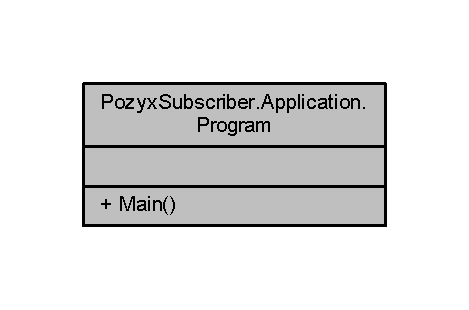
\includegraphics[width=225pt]{class_pozyx_subscriber_1_1_application_1_1_program__coll__graph}
\end{center}
\end{figure}
\subsection*{Static Public Member Functions}
\begin{DoxyCompactItemize}
\item 
static void \hyperlink{class_pozyx_subscriber_1_1_application_1_1_program_a35d33857544887b054b88bb37aeff83c}{Main} (string\mbox{[}$\,$\mbox{]} args)
\end{DoxyCompactItemize}


\subsection{Member Function Documentation}
\mbox{\Hypertarget{class_pozyx_subscriber_1_1_application_1_1_program_a35d33857544887b054b88bb37aeff83c}\label{class_pozyx_subscriber_1_1_application_1_1_program_a35d33857544887b054b88bb37aeff83c}} 
\index{Pozyx\+Subscriber\+::\+Application\+::\+Program@{Pozyx\+Subscriber\+::\+Application\+::\+Program}!Main@{Main}}
\index{Main@{Main}!Pozyx\+Subscriber\+::\+Application\+::\+Program@{Pozyx\+Subscriber\+::\+Application\+::\+Program}}
\subsubsection{\texorpdfstring{Main()}{Main()}}
{\footnotesize\ttfamily static void Pozyx\+Subscriber.\+Application.\+Program.\+Main (\begin{DoxyParamCaption}\item[{string \mbox{[}$\,$\mbox{]}}]{args }\end{DoxyParamCaption})\hspace{0.3cm}{\ttfamily [static]}}



The documentation for this class was generated from the following file\+:\begin{DoxyCompactItemize}
\item 
Project/\+Pozyx\+Subscriber/\+Pozyx\+Subscriber/\+Application/\hyperlink{_application_2_application_8cs}{Application.\+cs}\end{DoxyCompactItemize}

\hypertarget{class_pozyx_subscriber_1_1_framework_1_1_reader}{}\section{Pozyx\+Subscriber.\+Framework.\+Reader Class Reference}
\label{class_pozyx_subscriber_1_1_framework_1_1_reader}\index{Pozyx\+Subscriber.\+Framework.\+Reader@{Pozyx\+Subscriber.\+Framework.\+Reader}}


Mqqt client for subscribing to pozyx broker  




Collaboration diagram for Pozyx\+Subscriber.\+Framework.\+Reader\+:
% FIG 0
\subsection*{Public Member Functions}
\begin{DoxyCompactItemize}
\item 
\hyperlink{class_pozyx_subscriber_1_1_framework_1_1_reader_a34b6d7d372c71c7811229d42ce07e31f}{Reader} (string filename, \hyperlink{class_pozyx_subscriber_1_1_sim_environment}{Sim\+Environment} S)
\item 
void \hyperlink{class_pozyx_subscriber_1_1_framework_1_1_reader_afb1a43eb336971690e2c3fde43947b1d}{Begin} ()
\item 
async Task \hyperlink{class_pozyx_subscriber_1_1_framework_1_1_reader_a41ad44c9590bacac708e2ed4a24d56b2}{Start\+Async} ()
\end{DoxyCompactItemize}
\subsection*{Private Attributes}
\begin{DoxyCompactItemize}
\item 
\hyperlink{class_pozyx_subscriber_1_1_sim_environment}{Sim\+Environment} \hyperlink{class_pozyx_subscriber_1_1_framework_1_1_reader_a2105f5c7ce04e3a24ca3113f97f500b2}{\+\_\+sim}
\item 
string \hyperlink{class_pozyx_subscriber_1_1_framework_1_1_reader_ac76e24779e67f985f38d3d5070cb0535}{\+\_\+filename}
\item 
float \hyperlink{class_pozyx_subscriber_1_1_framework_1_1_reader_a19c48a4c5be9fb991299d29d7378bbee}{time}
\end{DoxyCompactItemize}


\subsection{Detailed Description}
Mqqt client for subscribing to pozyx broker 



\subsection{Constructor \& Destructor Documentation}
\mbox{\Hypertarget{class_pozyx_subscriber_1_1_framework_1_1_reader_a34b6d7d372c71c7811229d42ce07e31f}\label{class_pozyx_subscriber_1_1_framework_1_1_reader_a34b6d7d372c71c7811229d42ce07e31f}} 
\index{Pozyx\+Subscriber\+::\+Framework\+::\+Reader@{Pozyx\+Subscriber\+::\+Framework\+::\+Reader}!Reader@{Reader}}
\index{Reader@{Reader}!Pozyx\+Subscriber\+::\+Framework\+::\+Reader@{Pozyx\+Subscriber\+::\+Framework\+::\+Reader}}
\subsubsection{\texorpdfstring{Reader()}{Reader()}}
{\footnotesize\ttfamily Pozyx\+Subscriber.\+Framework.\+Reader.\+Reader (\begin{DoxyParamCaption}\item[{string}]{filename,  }\item[{\hyperlink{class_pozyx_subscriber_1_1_sim_environment}{Sim\+Environment}}]{S }\end{DoxyParamCaption})}



\subsection{Member Function Documentation}
\mbox{\Hypertarget{class_pozyx_subscriber_1_1_framework_1_1_reader_afb1a43eb336971690e2c3fde43947b1d}\label{class_pozyx_subscriber_1_1_framework_1_1_reader_afb1a43eb336971690e2c3fde43947b1d}} 
\index{Pozyx\+Subscriber\+::\+Framework\+::\+Reader@{Pozyx\+Subscriber\+::\+Framework\+::\+Reader}!Begin@{Begin}}
\index{Begin@{Begin}!Pozyx\+Subscriber\+::\+Framework\+::\+Reader@{Pozyx\+Subscriber\+::\+Framework\+::\+Reader}}
\subsubsection{\texorpdfstring{Begin()}{Begin()}}
{\footnotesize\ttfamily void Pozyx\+Subscriber.\+Framework.\+Reader.\+Begin (\begin{DoxyParamCaption}{ }\end{DoxyParamCaption})}

Here is the caller graph for this function\+:
% FIG 1
\mbox{\Hypertarget{class_pozyx_subscriber_1_1_framework_1_1_reader_a41ad44c9590bacac708e2ed4a24d56b2}\label{class_pozyx_subscriber_1_1_framework_1_1_reader_a41ad44c9590bacac708e2ed4a24d56b2}} 
\index{Pozyx\+Subscriber\+::\+Framework\+::\+Reader@{Pozyx\+Subscriber\+::\+Framework\+::\+Reader}!Start\+Async@{Start\+Async}}
\index{Start\+Async@{Start\+Async}!Pozyx\+Subscriber\+::\+Framework\+::\+Reader@{Pozyx\+Subscriber\+::\+Framework\+::\+Reader}}
\subsubsection{\texorpdfstring{Start\+Async()}{StartAsync()}}
{\footnotesize\ttfamily async Task Pozyx\+Subscriber.\+Framework.\+Reader.\+Start\+Async (\begin{DoxyParamCaption}{ }\end{DoxyParamCaption})}

Here is the call graph for this function\+:
% FIG 2


\subsection{Member Data Documentation}
\mbox{\Hypertarget{class_pozyx_subscriber_1_1_framework_1_1_reader_ac76e24779e67f985f38d3d5070cb0535}\label{class_pozyx_subscriber_1_1_framework_1_1_reader_ac76e24779e67f985f38d3d5070cb0535}} 
\index{Pozyx\+Subscriber\+::\+Framework\+::\+Reader@{Pozyx\+Subscriber\+::\+Framework\+::\+Reader}!\+\_\+filename@{\+\_\+filename}}
\index{\+\_\+filename@{\+\_\+filename}!Pozyx\+Subscriber\+::\+Framework\+::\+Reader@{Pozyx\+Subscriber\+::\+Framework\+::\+Reader}}
\subsubsection{\texorpdfstring{\+\_\+filename}{\_filename}}
{\footnotesize\ttfamily string Pozyx\+Subscriber.\+Framework.\+Reader.\+\_\+filename\hspace{0.3cm}{\ttfamily [private]}}

\mbox{\Hypertarget{class_pozyx_subscriber_1_1_framework_1_1_reader_a2105f5c7ce04e3a24ca3113f97f500b2}\label{class_pozyx_subscriber_1_1_framework_1_1_reader_a2105f5c7ce04e3a24ca3113f97f500b2}} 
\index{Pozyx\+Subscriber\+::\+Framework\+::\+Reader@{Pozyx\+Subscriber\+::\+Framework\+::\+Reader}!\+\_\+sim@{\+\_\+sim}}
\index{\+\_\+sim@{\+\_\+sim}!Pozyx\+Subscriber\+::\+Framework\+::\+Reader@{Pozyx\+Subscriber\+::\+Framework\+::\+Reader}}
\subsubsection{\texorpdfstring{\+\_\+sim}{\_sim}}
{\footnotesize\ttfamily \hyperlink{class_pozyx_subscriber_1_1_sim_environment}{Sim\+Environment} Pozyx\+Subscriber.\+Framework.\+Reader.\+\_\+sim\hspace{0.3cm}{\ttfamily [private]}}

\mbox{\Hypertarget{class_pozyx_subscriber_1_1_framework_1_1_reader_a19c48a4c5be9fb991299d29d7378bbee}\label{class_pozyx_subscriber_1_1_framework_1_1_reader_a19c48a4c5be9fb991299d29d7378bbee}} 
\index{Pozyx\+Subscriber\+::\+Framework\+::\+Reader@{Pozyx\+Subscriber\+::\+Framework\+::\+Reader}!time@{time}}
\index{time@{time}!Pozyx\+Subscriber\+::\+Framework\+::\+Reader@{Pozyx\+Subscriber\+::\+Framework\+::\+Reader}}
\subsubsection{\texorpdfstring{time}{time}}
{\footnotesize\ttfamily float Pozyx\+Subscriber.\+Framework.\+Reader.\+time\hspace{0.3cm}{\ttfamily [private]}}



The documentation for this class was generated from the following file\+:\begin{DoxyCompactItemize}
\item 
Project/\+Pozyx\+Subscriber/\+Pozyx\+Subscriber/\+Framework/\hyperlink{_file_reader_8cs}{File\+Reader.\+cs}\end{DoxyCompactItemize}

\hypertarget{class_pozyx_subscriber_1_1_sim_environment}{}\section{Pozyx\+Subscriber.\+Sim\+Environment Class Reference}
\label{class_pozyx_subscriber_1_1_sim_environment}\index{Pozyx\+Subscriber.\+Sim\+Environment@{Pozyx\+Subscriber.\+Sim\+Environment}}


Simulation enviornemnt  




Collaboration diagram for Pozyx\+Subscriber.\+Sim\+Environment\+:
\nopagebreak
\begin{figure}[H]
\begin{center}
\leavevmode
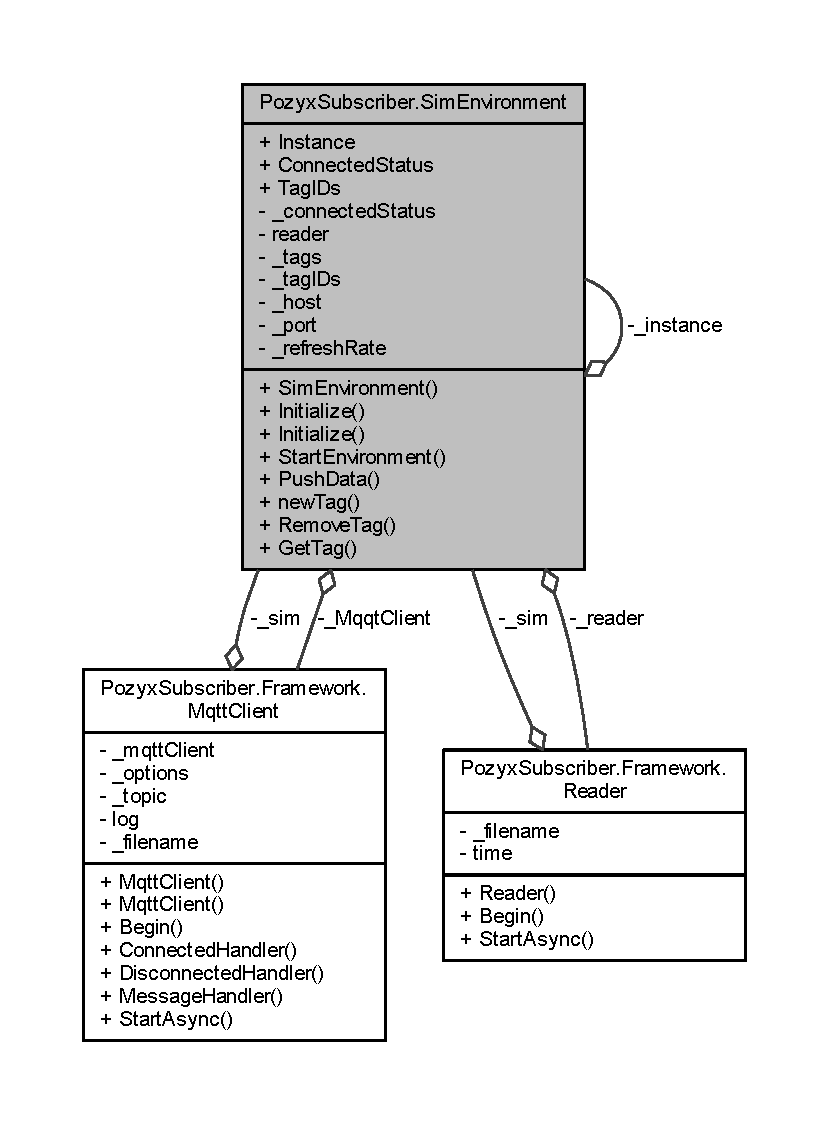
\includegraphics[width=350pt]{class_pozyx_subscriber_1_1_sim_environment__coll__graph}
\end{center}
\end{figure}
\subsection*{Public Member Functions}
\begin{DoxyCompactItemize}
\item 
\hyperlink{class_pozyx_subscriber_1_1_sim_environment_a3b5bc1fd7dd731dd19e3441c1ab0b54b}{Sim\+Environment} ()
\item 
void \hyperlink{class_pozyx_subscriber_1_1_sim_environment_a84c5b43571ebc24a983d38f8cfa219bf}{Initialize} (string host, int port, string filename, int refresh\+Rate)
\begin{DoxyCompactList}\small\item\em Simulation Enviorntment Constructor, creates Mqqt\+Client instance starting subscription to tags topic \end{DoxyCompactList}\item 
void \hyperlink{class_pozyx_subscriber_1_1_sim_environment_acfe443c048085a6f9873e87b43f0b6eb}{Initialize} (string filename, int refresh\+Rate)
\begin{DoxyCompactList}\small\item\em Simulation Enviorntment Constructor, creates reader instance will send J\+S\+ON strings in coordination to how P\+O\+Z\+YX does using a log file. Simulates reciving tag reads in realtime using a historic log \end{DoxyCompactList}\item 
void \hyperlink{class_pozyx_subscriber_1_1_sim_environment_a1804d91547ecc65c02091d63e8c1163e}{Start\+Environment} ()
\begin{DoxyCompactList}\small\item\em Start\+Environment method, will begin tracking/reading J\+S\+ON strings and tag readings from Pozyx on a separate thread This begins populating the simulation environment \end{DoxyCompactList}\item 
void \hyperlink{class_pozyx_subscriber_1_1_sim_environment_abd4106d662f4991da45aa743b24c4d88}{Push\+Data} (J\+Array msgdata)
\begin{DoxyCompactList}\small\item\em Pushes a J\+S\+ON J\+Array into the simulation \end{DoxyCompactList}\item 
\hyperlink{class_pozyx_subscriber_1_1_framework_1_1_tag}{Tag} \hyperlink{class_pozyx_subscriber_1_1_sim_environment_af4ddb163b4b711c2c1105c7fc0253af9}{new\+Tag} (string ID, int refresh\+Rate)
\begin{DoxyCompactList}\small\item\em Adds a new tag to the simulation environment \end{DoxyCompactList}\item 
\hyperlink{class_pozyx_subscriber_1_1_framework_1_1_tag}{Tag} \hyperlink{class_pozyx_subscriber_1_1_sim_environment_a6386074fe09ea029c9203bd5cb969650}{Remove\+Tag} (string ID)
\begin{DoxyCompactList}\small\item\em Removes a tag from the simulation environment \end{DoxyCompactList}\item 
\hyperlink{class_pozyx_subscriber_1_1_framework_1_1_tag}{Tag} \hyperlink{class_pozyx_subscriber_1_1_sim_environment_aafaa3f130c9a8cc0a0eacb29253fbd7d}{Get\+Tag} (string ID)
\begin{DoxyCompactList}\small\item\em gets a tag from the simulation environment \end{DoxyCompactList}\end{DoxyCompactItemize}
\subsection*{Properties}
\begin{DoxyCompactItemize}
\item 
static \hyperlink{class_pozyx_subscriber_1_1_sim_environment}{Sim\+Environment} \hyperlink{class_pozyx_subscriber_1_1_sim_environment_a57d7b43dd1ff01a963153b24a79649a4}{Instance}\hspace{0.3cm}{\ttfamily  \mbox{[}get\mbox{]}}
\item 
bool \hyperlink{class_pozyx_subscriber_1_1_sim_environment_a32da22171f3ba4173336035846e3c170}{Connected\+Status}\hspace{0.3cm}{\ttfamily  \mbox{[}get, set\mbox{]}}
\begin{DoxyCompactList}\small\item\em The Connection status of the M\+Q\+TT or Reader class \end{DoxyCompactList}\item 
List$<$ string $>$ \hyperlink{class_pozyx_subscriber_1_1_sim_environment_a7395c9fc1afe5a0686f2b6693eef748b}{Tag\+I\+Ds}\hspace{0.3cm}{\ttfamily  \mbox{[}get\mbox{]}}
\begin{DoxyCompactList}\small\item\em a list of strings that contain the I\+Ds of all the active tags in the Simulation Environment \end{DoxyCompactList}\end{DoxyCompactItemize}
\subsection*{Private Attributes}
\begin{DoxyCompactItemize}
\item 
bool \hyperlink{class_pozyx_subscriber_1_1_sim_environment_a71e86b3047a367d0bfd08c92ce480509}{\+\_\+connected\+Status}
\item 
bool \hyperlink{class_pozyx_subscriber_1_1_sim_environment_a85870c67295486d7abb27f35603a4356}{reader}
\item 
\hyperlink{class_pozyx_subscriber_1_1_framework_1_1_reader}{Reader} \hyperlink{class_pozyx_subscriber_1_1_sim_environment_a97683f60e678f6552639b2d79d31cf3d}{\+\_\+reader}
\item 
Dictionary$<$ string, \hyperlink{class_pozyx_subscriber_1_1_framework_1_1_tag}{Tag} $>$ \hyperlink{class_pozyx_subscriber_1_1_sim_environment_a7a9050254e24024b517089b736316881}{\+\_\+tags}
\item 
List$<$ string $>$ \hyperlink{class_pozyx_subscriber_1_1_sim_environment_a726825a7059b308b64e9bc3787808327}{\+\_\+tag\+I\+Ds}
\item 
string \hyperlink{class_pozyx_subscriber_1_1_sim_environment_a40a0a0fd989252d51605ba77653818c8}{\+\_\+host}
\item 
int \hyperlink{class_pozyx_subscriber_1_1_sim_environment_a5667a6367405f1c0a2ffe300f4245590}{\+\_\+port}
\item 
int \hyperlink{class_pozyx_subscriber_1_1_sim_environment_a45020f3e4a891fdb094d5dc29cfe8291}{\+\_\+refresh\+Rate}
\end{DoxyCompactItemize}
\subsection*{Static Private Attributes}
\begin{DoxyCompactItemize}
\item 
static \hyperlink{class_pozyx_subscriber_1_1_sim_environment}{Sim\+Environment} \hyperlink{class_pozyx_subscriber_1_1_sim_environment_a5d5b39ad30ad8758fb7f53aaa50fc1fb}{\+\_\+instance} = null
\item 
static \hyperlink{class_pozyx_subscriber_1_1_framework_1_1_mqtt_client}{Mqtt\+Client} \hyperlink{class_pozyx_subscriber_1_1_sim_environment_a391436676bf93116d83dd7c422c5b8cd}{\+\_\+\+Mqqt\+Client}
\end{DoxyCompactItemize}


\subsection{Detailed Description}
Simulation enviornemnt 



\subsection{Constructor \& Destructor Documentation}
\mbox{\Hypertarget{class_pozyx_subscriber_1_1_sim_environment_a3b5bc1fd7dd731dd19e3441c1ab0b54b}\label{class_pozyx_subscriber_1_1_sim_environment_a3b5bc1fd7dd731dd19e3441c1ab0b54b}} 
\index{Pozyx\+Subscriber\+::\+Sim\+Environment@{Pozyx\+Subscriber\+::\+Sim\+Environment}!Sim\+Environment@{Sim\+Environment}}
\index{Sim\+Environment@{Sim\+Environment}!Pozyx\+Subscriber\+::\+Sim\+Environment@{Pozyx\+Subscriber\+::\+Sim\+Environment}}
\subsubsection{\texorpdfstring{Sim\+Environment()}{SimEnvironment()}}
{\footnotesize\ttfamily Pozyx\+Subscriber.\+Sim\+Environment.\+Sim\+Environment (\begin{DoxyParamCaption}{ }\end{DoxyParamCaption})}



\subsection{Member Function Documentation}
\mbox{\Hypertarget{class_pozyx_subscriber_1_1_sim_environment_aafaa3f130c9a8cc0a0eacb29253fbd7d}\label{class_pozyx_subscriber_1_1_sim_environment_aafaa3f130c9a8cc0a0eacb29253fbd7d}} 
\index{Pozyx\+Subscriber\+::\+Sim\+Environment@{Pozyx\+Subscriber\+::\+Sim\+Environment}!Get\+Tag@{Get\+Tag}}
\index{Get\+Tag@{Get\+Tag}!Pozyx\+Subscriber\+::\+Sim\+Environment@{Pozyx\+Subscriber\+::\+Sim\+Environment}}
\subsubsection{\texorpdfstring{Get\+Tag()}{GetTag()}}
{\footnotesize\ttfamily \hyperlink{class_pozyx_subscriber_1_1_framework_1_1_tag}{Tag} Pozyx\+Subscriber.\+Sim\+Environment.\+Get\+Tag (\begin{DoxyParamCaption}\item[{string}]{ID }\end{DoxyParamCaption})}



gets a tag from the simulation environment 


\begin{DoxyParams}{Parameters}
{\em ID} & the ID of the tag to get\\
\hline
\end{DoxyParams}
\begin{DoxyReturn}{Returns}
the requested tag 
\end{DoxyReturn}
\mbox{\Hypertarget{class_pozyx_subscriber_1_1_sim_environment_a84c5b43571ebc24a983d38f8cfa219bf}\label{class_pozyx_subscriber_1_1_sim_environment_a84c5b43571ebc24a983d38f8cfa219bf}} 
\index{Pozyx\+Subscriber\+::\+Sim\+Environment@{Pozyx\+Subscriber\+::\+Sim\+Environment}!Initialize@{Initialize}}
\index{Initialize@{Initialize}!Pozyx\+Subscriber\+::\+Sim\+Environment@{Pozyx\+Subscriber\+::\+Sim\+Environment}}
\subsubsection{\texorpdfstring{Initialize()}{Initialize()}\hspace{0.1cm}{\footnotesize\ttfamily [1/2]}}
{\footnotesize\ttfamily void Pozyx\+Subscriber.\+Sim\+Environment.\+Initialize (\begin{DoxyParamCaption}\item[{string}]{host,  }\item[{int}]{port,  }\item[{string}]{filename,  }\item[{int}]{refresh\+Rate }\end{DoxyParamCaption})}



Simulation Enviorntment Constructor, creates Mqqt\+Client instance starting subscription to tags topic 


\begin{DoxyParams}{Parameters}
{\em host} & Local IP addres of Pozyx gateway\\
\hline
{\em port} & Port\\
\hline
{\em filename} & a log file to keep track of all tag messages\\
\hline
{\em refresh\+Rate} & Default refresh rate of a tag not specified by the user\\
\hline
\end{DoxyParams}
Here is the caller graph for this function\+:
\nopagebreak
\begin{figure}[H]
\begin{center}
\leavevmode
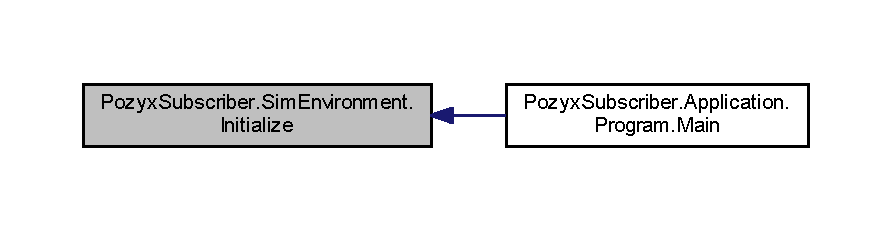
\includegraphics[width=350pt]{class_pozyx_subscriber_1_1_sim_environment_a84c5b43571ebc24a983d38f8cfa219bf_icgraph}
\end{center}
\end{figure}
\mbox{\Hypertarget{class_pozyx_subscriber_1_1_sim_environment_acfe443c048085a6f9873e87b43f0b6eb}\label{class_pozyx_subscriber_1_1_sim_environment_acfe443c048085a6f9873e87b43f0b6eb}} 
\index{Pozyx\+Subscriber\+::\+Sim\+Environment@{Pozyx\+Subscriber\+::\+Sim\+Environment}!Initialize@{Initialize}}
\index{Initialize@{Initialize}!Pozyx\+Subscriber\+::\+Sim\+Environment@{Pozyx\+Subscriber\+::\+Sim\+Environment}}
\subsubsection{\texorpdfstring{Initialize()}{Initialize()}\hspace{0.1cm}{\footnotesize\ttfamily [2/2]}}
{\footnotesize\ttfamily void Pozyx\+Subscriber.\+Sim\+Environment.\+Initialize (\begin{DoxyParamCaption}\item[{string}]{filename,  }\item[{int}]{refresh\+Rate }\end{DoxyParamCaption})}



Simulation Enviorntment Constructor, creates reader instance will send J\+S\+ON strings in coordination to how P\+O\+Z\+YX does using a log file. Simulates reciving tag reads in realtime using a historic log 


\begin{DoxyParams}{Parameters}
{\em filename} & name of the log file to simulate with\\
\hline
{\em refresh\+Rate} & Default refresh rate of a tag not specified by the user\\
\hline
\end{DoxyParams}
\mbox{\Hypertarget{class_pozyx_subscriber_1_1_sim_environment_af4ddb163b4b711c2c1105c7fc0253af9}\label{class_pozyx_subscriber_1_1_sim_environment_af4ddb163b4b711c2c1105c7fc0253af9}} 
\index{Pozyx\+Subscriber\+::\+Sim\+Environment@{Pozyx\+Subscriber\+::\+Sim\+Environment}!new\+Tag@{new\+Tag}}
\index{new\+Tag@{new\+Tag}!Pozyx\+Subscriber\+::\+Sim\+Environment@{Pozyx\+Subscriber\+::\+Sim\+Environment}}
\subsubsection{\texorpdfstring{new\+Tag()}{newTag()}}
{\footnotesize\ttfamily \hyperlink{class_pozyx_subscriber_1_1_framework_1_1_tag}{Tag} Pozyx\+Subscriber.\+Sim\+Environment.\+new\+Tag (\begin{DoxyParamCaption}\item[{string}]{ID,  }\item[{int}]{refresh\+Rate }\end{DoxyParamCaption})}



Adds a new tag to the simulation environment 


\begin{DoxyParams}{Parameters}
{\em ID} & the ID of the tag to add\\
\hline
{\em refresh\+Rate} & the refresh rate of the added tag\\
\hline
\end{DoxyParams}
\begin{DoxyReturn}{Returns}
the newly created tag 
\end{DoxyReturn}
Here is the caller graph for this function\+:
\nopagebreak
\begin{figure}[H]
\begin{center}
\leavevmode
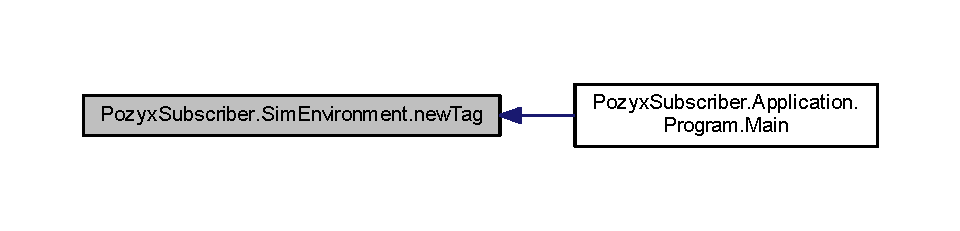
\includegraphics[width=350pt]{class_pozyx_subscriber_1_1_sim_environment_af4ddb163b4b711c2c1105c7fc0253af9_icgraph}
\end{center}
\end{figure}
\mbox{\Hypertarget{class_pozyx_subscriber_1_1_sim_environment_abd4106d662f4991da45aa743b24c4d88}\label{class_pozyx_subscriber_1_1_sim_environment_abd4106d662f4991da45aa743b24c4d88}} 
\index{Pozyx\+Subscriber\+::\+Sim\+Environment@{Pozyx\+Subscriber\+::\+Sim\+Environment}!Push\+Data@{Push\+Data}}
\index{Push\+Data@{Push\+Data}!Pozyx\+Subscriber\+::\+Sim\+Environment@{Pozyx\+Subscriber\+::\+Sim\+Environment}}
\subsubsection{\texorpdfstring{Push\+Data()}{PushData()}}
{\footnotesize\ttfamily void Pozyx\+Subscriber.\+Sim\+Environment.\+Push\+Data (\begin{DoxyParamCaption}\item[{J\+Array}]{msgdata }\end{DoxyParamCaption})}



Pushes a J\+S\+ON J\+Array into the simulation 


\begin{DoxyParams}{Parameters}
{\em msgdata} & the J\+Array parsed to populate the simulation environment with\\
\hline
\end{DoxyParams}
Here is the caller graph for this function\+:
\nopagebreak
\begin{figure}[H]
\begin{center}
\leavevmode
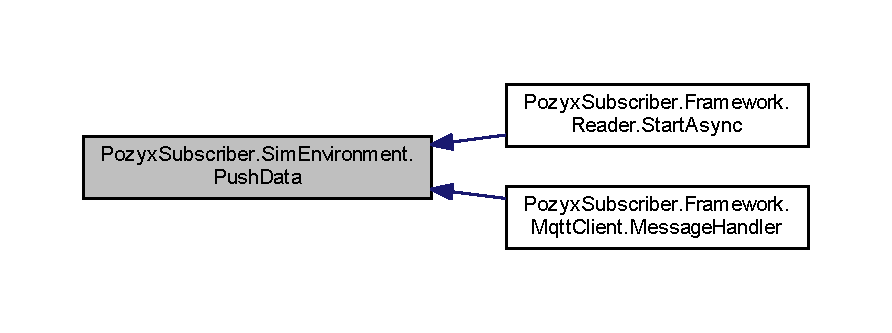
\includegraphics[width=350pt]{class_pozyx_subscriber_1_1_sim_environment_abd4106d662f4991da45aa743b24c4d88_icgraph}
\end{center}
\end{figure}
\mbox{\Hypertarget{class_pozyx_subscriber_1_1_sim_environment_a6386074fe09ea029c9203bd5cb969650}\label{class_pozyx_subscriber_1_1_sim_environment_a6386074fe09ea029c9203bd5cb969650}} 
\index{Pozyx\+Subscriber\+::\+Sim\+Environment@{Pozyx\+Subscriber\+::\+Sim\+Environment}!Remove\+Tag@{Remove\+Tag}}
\index{Remove\+Tag@{Remove\+Tag}!Pozyx\+Subscriber\+::\+Sim\+Environment@{Pozyx\+Subscriber\+::\+Sim\+Environment}}
\subsubsection{\texorpdfstring{Remove\+Tag()}{RemoveTag()}}
{\footnotesize\ttfamily \hyperlink{class_pozyx_subscriber_1_1_framework_1_1_tag}{Tag} Pozyx\+Subscriber.\+Sim\+Environment.\+Remove\+Tag (\begin{DoxyParamCaption}\item[{string}]{ID }\end{DoxyParamCaption})}



Removes a tag from the simulation environment 


\begin{DoxyParams}{Parameters}
{\em ID} & the ID of the tag to remove\\
\hline
\end{DoxyParams}
\begin{DoxyReturn}{Returns}
the removed tag 
\end{DoxyReturn}
\mbox{\Hypertarget{class_pozyx_subscriber_1_1_sim_environment_a1804d91547ecc65c02091d63e8c1163e}\label{class_pozyx_subscriber_1_1_sim_environment_a1804d91547ecc65c02091d63e8c1163e}} 
\index{Pozyx\+Subscriber\+::\+Sim\+Environment@{Pozyx\+Subscriber\+::\+Sim\+Environment}!Start\+Environment@{Start\+Environment}}
\index{Start\+Environment@{Start\+Environment}!Pozyx\+Subscriber\+::\+Sim\+Environment@{Pozyx\+Subscriber\+::\+Sim\+Environment}}
\subsubsection{\texorpdfstring{Start\+Environment()}{StartEnvironment()}}
{\footnotesize\ttfamily void Pozyx\+Subscriber.\+Sim\+Environment.\+Start\+Environment (\begin{DoxyParamCaption}{ }\end{DoxyParamCaption})}



Start\+Environment method, will begin tracking/reading J\+S\+ON strings and tag readings from Pozyx on a separate thread This begins populating the simulation environment 

Here is the call graph for this function\+:
\nopagebreak
\begin{figure}[H]
\begin{center}
\leavevmode
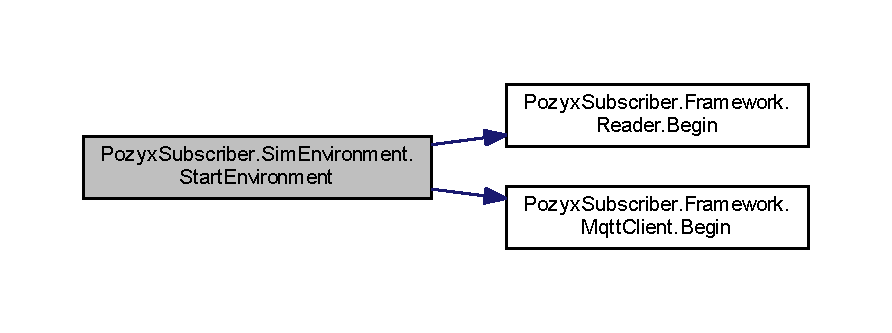
\includegraphics[width=350pt]{class_pozyx_subscriber_1_1_sim_environment_a1804d91547ecc65c02091d63e8c1163e_cgraph}
\end{center}
\end{figure}
Here is the caller graph for this function\+:
\nopagebreak
\begin{figure}[H]
\begin{center}
\leavevmode
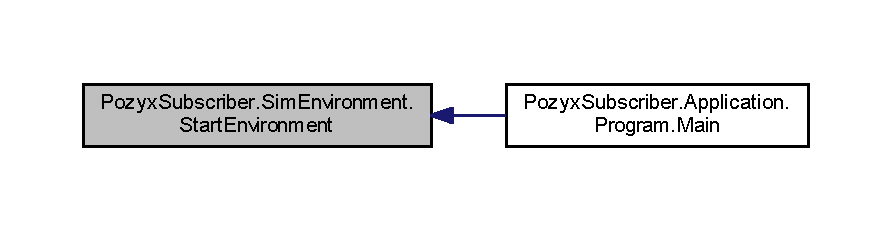
\includegraphics[width=350pt]{class_pozyx_subscriber_1_1_sim_environment_a1804d91547ecc65c02091d63e8c1163e_icgraph}
\end{center}
\end{figure}


\subsection{Member Data Documentation}
\mbox{\Hypertarget{class_pozyx_subscriber_1_1_sim_environment_a71e86b3047a367d0bfd08c92ce480509}\label{class_pozyx_subscriber_1_1_sim_environment_a71e86b3047a367d0bfd08c92ce480509}} 
\index{Pozyx\+Subscriber\+::\+Sim\+Environment@{Pozyx\+Subscriber\+::\+Sim\+Environment}!\+\_\+connected\+Status@{\+\_\+connected\+Status}}
\index{\+\_\+connected\+Status@{\+\_\+connected\+Status}!Pozyx\+Subscriber\+::\+Sim\+Environment@{Pozyx\+Subscriber\+::\+Sim\+Environment}}
\subsubsection{\texorpdfstring{\+\_\+connected\+Status}{\_connectedStatus}}
{\footnotesize\ttfamily bool Pozyx\+Subscriber.\+Sim\+Environment.\+\_\+connected\+Status\hspace{0.3cm}{\ttfamily [private]}}

\mbox{\Hypertarget{class_pozyx_subscriber_1_1_sim_environment_a40a0a0fd989252d51605ba77653818c8}\label{class_pozyx_subscriber_1_1_sim_environment_a40a0a0fd989252d51605ba77653818c8}} 
\index{Pozyx\+Subscriber\+::\+Sim\+Environment@{Pozyx\+Subscriber\+::\+Sim\+Environment}!\+\_\+host@{\+\_\+host}}
\index{\+\_\+host@{\+\_\+host}!Pozyx\+Subscriber\+::\+Sim\+Environment@{Pozyx\+Subscriber\+::\+Sim\+Environment}}
\subsubsection{\texorpdfstring{\+\_\+host}{\_host}}
{\footnotesize\ttfamily string Pozyx\+Subscriber.\+Sim\+Environment.\+\_\+host\hspace{0.3cm}{\ttfamily [private]}}

\mbox{\Hypertarget{class_pozyx_subscriber_1_1_sim_environment_a5d5b39ad30ad8758fb7f53aaa50fc1fb}\label{class_pozyx_subscriber_1_1_sim_environment_a5d5b39ad30ad8758fb7f53aaa50fc1fb}} 
\index{Pozyx\+Subscriber\+::\+Sim\+Environment@{Pozyx\+Subscriber\+::\+Sim\+Environment}!\+\_\+instance@{\+\_\+instance}}
\index{\+\_\+instance@{\+\_\+instance}!Pozyx\+Subscriber\+::\+Sim\+Environment@{Pozyx\+Subscriber\+::\+Sim\+Environment}}
\subsubsection{\texorpdfstring{\+\_\+instance}{\_instance}}
{\footnotesize\ttfamily \hyperlink{class_pozyx_subscriber_1_1_sim_environment}{Sim\+Environment} Pozyx\+Subscriber.\+Sim\+Environment.\+\_\+instance = null\hspace{0.3cm}{\ttfamily [static]}, {\ttfamily [private]}}

\mbox{\Hypertarget{class_pozyx_subscriber_1_1_sim_environment_a391436676bf93116d83dd7c422c5b8cd}\label{class_pozyx_subscriber_1_1_sim_environment_a391436676bf93116d83dd7c422c5b8cd}} 
\index{Pozyx\+Subscriber\+::\+Sim\+Environment@{Pozyx\+Subscriber\+::\+Sim\+Environment}!\+\_\+\+Mqqt\+Client@{\+\_\+\+Mqqt\+Client}}
\index{\+\_\+\+Mqqt\+Client@{\+\_\+\+Mqqt\+Client}!Pozyx\+Subscriber\+::\+Sim\+Environment@{Pozyx\+Subscriber\+::\+Sim\+Environment}}
\subsubsection{\texorpdfstring{\+\_\+\+Mqqt\+Client}{\_MqqtClient}}
{\footnotesize\ttfamily \hyperlink{class_pozyx_subscriber_1_1_framework_1_1_mqtt_client}{Mqtt\+Client} Pozyx\+Subscriber.\+Sim\+Environment.\+\_\+\+Mqqt\+Client\hspace{0.3cm}{\ttfamily [static]}, {\ttfamily [private]}}

\mbox{\Hypertarget{class_pozyx_subscriber_1_1_sim_environment_a5667a6367405f1c0a2ffe300f4245590}\label{class_pozyx_subscriber_1_1_sim_environment_a5667a6367405f1c0a2ffe300f4245590}} 
\index{Pozyx\+Subscriber\+::\+Sim\+Environment@{Pozyx\+Subscriber\+::\+Sim\+Environment}!\+\_\+port@{\+\_\+port}}
\index{\+\_\+port@{\+\_\+port}!Pozyx\+Subscriber\+::\+Sim\+Environment@{Pozyx\+Subscriber\+::\+Sim\+Environment}}
\subsubsection{\texorpdfstring{\+\_\+port}{\_port}}
{\footnotesize\ttfamily int Pozyx\+Subscriber.\+Sim\+Environment.\+\_\+port\hspace{0.3cm}{\ttfamily [private]}}

\mbox{\Hypertarget{class_pozyx_subscriber_1_1_sim_environment_a97683f60e678f6552639b2d79d31cf3d}\label{class_pozyx_subscriber_1_1_sim_environment_a97683f60e678f6552639b2d79d31cf3d}} 
\index{Pozyx\+Subscriber\+::\+Sim\+Environment@{Pozyx\+Subscriber\+::\+Sim\+Environment}!\+\_\+reader@{\+\_\+reader}}
\index{\+\_\+reader@{\+\_\+reader}!Pozyx\+Subscriber\+::\+Sim\+Environment@{Pozyx\+Subscriber\+::\+Sim\+Environment}}
\subsubsection{\texorpdfstring{\+\_\+reader}{\_reader}}
{\footnotesize\ttfamily \hyperlink{class_pozyx_subscriber_1_1_framework_1_1_reader}{Reader} Pozyx\+Subscriber.\+Sim\+Environment.\+\_\+reader\hspace{0.3cm}{\ttfamily [private]}}

\mbox{\Hypertarget{class_pozyx_subscriber_1_1_sim_environment_a45020f3e4a891fdb094d5dc29cfe8291}\label{class_pozyx_subscriber_1_1_sim_environment_a45020f3e4a891fdb094d5dc29cfe8291}} 
\index{Pozyx\+Subscriber\+::\+Sim\+Environment@{Pozyx\+Subscriber\+::\+Sim\+Environment}!\+\_\+refresh\+Rate@{\+\_\+refresh\+Rate}}
\index{\+\_\+refresh\+Rate@{\+\_\+refresh\+Rate}!Pozyx\+Subscriber\+::\+Sim\+Environment@{Pozyx\+Subscriber\+::\+Sim\+Environment}}
\subsubsection{\texorpdfstring{\+\_\+refresh\+Rate}{\_refreshRate}}
{\footnotesize\ttfamily int Pozyx\+Subscriber.\+Sim\+Environment.\+\_\+refresh\+Rate\hspace{0.3cm}{\ttfamily [private]}}

\mbox{\Hypertarget{class_pozyx_subscriber_1_1_sim_environment_a726825a7059b308b64e9bc3787808327}\label{class_pozyx_subscriber_1_1_sim_environment_a726825a7059b308b64e9bc3787808327}} 
\index{Pozyx\+Subscriber\+::\+Sim\+Environment@{Pozyx\+Subscriber\+::\+Sim\+Environment}!\+\_\+tag\+I\+Ds@{\+\_\+tag\+I\+Ds}}
\index{\+\_\+tag\+I\+Ds@{\+\_\+tag\+I\+Ds}!Pozyx\+Subscriber\+::\+Sim\+Environment@{Pozyx\+Subscriber\+::\+Sim\+Environment}}
\subsubsection{\texorpdfstring{\+\_\+tag\+I\+Ds}{\_tagIDs}}
{\footnotesize\ttfamily List$<$string$>$ Pozyx\+Subscriber.\+Sim\+Environment.\+\_\+tag\+I\+Ds\hspace{0.3cm}{\ttfamily [private]}}

\mbox{\Hypertarget{class_pozyx_subscriber_1_1_sim_environment_a7a9050254e24024b517089b736316881}\label{class_pozyx_subscriber_1_1_sim_environment_a7a9050254e24024b517089b736316881}} 
\index{Pozyx\+Subscriber\+::\+Sim\+Environment@{Pozyx\+Subscriber\+::\+Sim\+Environment}!\+\_\+tags@{\+\_\+tags}}
\index{\+\_\+tags@{\+\_\+tags}!Pozyx\+Subscriber\+::\+Sim\+Environment@{Pozyx\+Subscriber\+::\+Sim\+Environment}}
\subsubsection{\texorpdfstring{\+\_\+tags}{\_tags}}
{\footnotesize\ttfamily Dictionary$<$string, \hyperlink{class_pozyx_subscriber_1_1_framework_1_1_tag}{Tag}$>$ Pozyx\+Subscriber.\+Sim\+Environment.\+\_\+tags\hspace{0.3cm}{\ttfamily [private]}}

\mbox{\Hypertarget{class_pozyx_subscriber_1_1_sim_environment_a85870c67295486d7abb27f35603a4356}\label{class_pozyx_subscriber_1_1_sim_environment_a85870c67295486d7abb27f35603a4356}} 
\index{Pozyx\+Subscriber\+::\+Sim\+Environment@{Pozyx\+Subscriber\+::\+Sim\+Environment}!reader@{reader}}
\index{reader@{reader}!Pozyx\+Subscriber\+::\+Sim\+Environment@{Pozyx\+Subscriber\+::\+Sim\+Environment}}
\subsubsection{\texorpdfstring{reader}{reader}}
{\footnotesize\ttfamily bool Pozyx\+Subscriber.\+Sim\+Environment.\+reader\hspace{0.3cm}{\ttfamily [private]}}



\subsection{Property Documentation}
\mbox{\Hypertarget{class_pozyx_subscriber_1_1_sim_environment_a32da22171f3ba4173336035846e3c170}\label{class_pozyx_subscriber_1_1_sim_environment_a32da22171f3ba4173336035846e3c170}} 
\index{Pozyx\+Subscriber\+::\+Sim\+Environment@{Pozyx\+Subscriber\+::\+Sim\+Environment}!Connected\+Status@{Connected\+Status}}
\index{Connected\+Status@{Connected\+Status}!Pozyx\+Subscriber\+::\+Sim\+Environment@{Pozyx\+Subscriber\+::\+Sim\+Environment}}
\subsubsection{\texorpdfstring{Connected\+Status}{ConnectedStatus}}
{\footnotesize\ttfamily bool Pozyx\+Subscriber.\+Sim\+Environment.\+Connected\+Status\hspace{0.3cm}{\ttfamily [get]}, {\ttfamily [set]}}



The Connection status of the M\+Q\+TT or Reader class 

\mbox{\Hypertarget{class_pozyx_subscriber_1_1_sim_environment_a57d7b43dd1ff01a963153b24a79649a4}\label{class_pozyx_subscriber_1_1_sim_environment_a57d7b43dd1ff01a963153b24a79649a4}} 
\index{Pozyx\+Subscriber\+::\+Sim\+Environment@{Pozyx\+Subscriber\+::\+Sim\+Environment}!Instance@{Instance}}
\index{Instance@{Instance}!Pozyx\+Subscriber\+::\+Sim\+Environment@{Pozyx\+Subscriber\+::\+Sim\+Environment}}
\subsubsection{\texorpdfstring{Instance}{Instance}}
{\footnotesize\ttfamily \hyperlink{class_pozyx_subscriber_1_1_sim_environment}{Sim\+Environment} Pozyx\+Subscriber.\+Sim\+Environment.\+Instance\hspace{0.3cm}{\ttfamily [static]}, {\ttfamily [get]}}

\mbox{\Hypertarget{class_pozyx_subscriber_1_1_sim_environment_a7395c9fc1afe5a0686f2b6693eef748b}\label{class_pozyx_subscriber_1_1_sim_environment_a7395c9fc1afe5a0686f2b6693eef748b}} 
\index{Pozyx\+Subscriber\+::\+Sim\+Environment@{Pozyx\+Subscriber\+::\+Sim\+Environment}!Tag\+I\+Ds@{Tag\+I\+Ds}}
\index{Tag\+I\+Ds@{Tag\+I\+Ds}!Pozyx\+Subscriber\+::\+Sim\+Environment@{Pozyx\+Subscriber\+::\+Sim\+Environment}}
\subsubsection{\texorpdfstring{Tag\+I\+Ds}{TagIDs}}
{\footnotesize\ttfamily List$<$string$>$ Pozyx\+Subscriber.\+Sim\+Environment.\+Tag\+I\+Ds\hspace{0.3cm}{\ttfamily [get]}}



a list of strings that contain the I\+Ds of all the active tags in the Simulation Environment 



The documentation for this class was generated from the following file\+:\begin{DoxyCompactItemize}
\item 
Project/\+Pozyx\+Subscriber/\+Pozyx\+Subscriber/\hyperlink{_simulation_environment_8cs}{Simulation\+Environment.\+cs}\end{DoxyCompactItemize}

\hypertarget{class_pozyx_subscriber_1_1_framework_1_1_sim_object}{}\section{Pozyx\+Subscriber.\+Framework.\+Sim\+Object Class Reference}
\label{class_pozyx_subscriber_1_1_framework_1_1_sim_object}\index{Pozyx\+Subscriber.\+Framework.\+Sim\+Object@{Pozyx\+Subscriber.\+Framework.\+Sim\+Object}}


Collaboration diagram for Pozyx\+Subscriber.\+Framework.\+Sim\+Object\+:
% FIG 0
\subsection*{Public Member Functions}
\begin{DoxyCompactItemize}
\item 
\hyperlink{class_pozyx_subscriber_1_1_framework_1_1_sim_object_ab0a3cd312e9fdd62beea5f4dd5ecbd7f}{Sim\+Object} ()
\begin{DoxyCompactList}\small\item\em \hyperlink{class_pozyx_subscriber_1_1_framework_1_1_sim_object}{Sim\+Object} Constructor \end{DoxyCompactList}\item 
bool \hyperlink{class_pozyx_subscriber_1_1_framework_1_1_sim_object_a54c41e58e89d8ed0c99f4438decbeb2c}{Contains} (\hyperlink{class_pozyx_subscriber_1_1_framework_1_1_tag}{Tag} tag)
\begin{DoxyCompactList}\small\item\em Checks to see if this \hyperlink{class_pozyx_subscriber_1_1_framework_1_1_sim_object}{Sim\+Object} has a specific tag attached to it \end{DoxyCompactList}\item 
void \hyperlink{class_pozyx_subscriber_1_1_framework_1_1_sim_object_a9cac7e5ea0f5e6e5d0018a62ae055de0}{Add\+Tag} (\hyperlink{class_pozyx_subscriber_1_1_framework_1_1_tag}{Tag} tag)
\begin{DoxyCompactList}\small\item\em attaches a tag to this object for tracking, maximum of 2 tags must be attached for orientation measurements \end{DoxyCompactList}\item 
void \hyperlink{class_pozyx_subscriber_1_1_framework_1_1_sim_object_a4b3f38bbd3d9ad1b621f08c2317d66f8}{remove\+Tag} (\hyperlink{class_pozyx_subscriber_1_1_framework_1_1_tag}{Tag} tag)
\begin{DoxyCompactList}\small\item\em removes a tag from this object \end{DoxyCompactList}\item 
void \hyperlink{class_pozyx_subscriber_1_1_framework_1_1_sim_object_a1c648d512ff2292a3f0f084f54ab9cae}{Calibrate} (\hyperlink{class_pozyx_subscriber_1_1_sim_environment}{Sim\+Environment} S)
\begin{DoxyCompactList}\small\item\em sets the \hyperlink{class_pozyx_subscriber_1_1_framework_1_1_sim_object}{Sim\+Object}\textquotesingle{}s current position and orientation in the real world be the default 0, and reinitializes its coordinate readings. Must be done after attaching tags to a \hyperlink{class_pozyx_subscriber_1_1_framework_1_1_sim_object}{Sim\+Object}, Simulation\+Environment must be running \end{DoxyCompactList}\item 
void \hyperlink{class_pozyx_subscriber_1_1_framework_1_1_sim_object_abf399bdb3a84bd97df64b9cf47482cbd}{Calibrate} (\hyperlink{class_pozyx_subscriber_1_1_sim_environment}{Sim\+Environment} S, float xpos, float ypos, float zpos)
\begin{DoxyCompactList}\small\item\em sets the \hyperlink{class_pozyx_subscriber_1_1_framework_1_1_sim_object}{Sim\+Object}\textquotesingle{}s current position in the real world be the set pos values, and reinitializes its coordinate readings. Sets current real world orientation to 0 Must be done after attaching tags to a \hyperlink{class_pozyx_subscriber_1_1_framework_1_1_sim_object}{Sim\+Object}, Simulation\+Environment must be running and connected \end{DoxyCompactList}\end{DoxyCompactItemize}
\subsection*{Properties}
\begin{DoxyCompactItemize}
\item 
\hyperlink{struct_pozyx_subscriber_1_1_framework_1_1_pozyx_vector}{Pozyx\+Vector} \hyperlink{class_pozyx_subscriber_1_1_framework_1_1_sim_object_a154ba70dc97ab79384ebecae98d69e18}{Position}\hspace{0.3cm}{\ttfamily  \mbox{[}get\mbox{]}}
\begin{DoxyCompactList}\small\item\em \hyperlink{struct_pozyx_subscriber_1_1_framework_1_1_pozyx_vector}{Pozyx\+Vector}\+: The Position of the current Simobject \end{DoxyCompactList}\item 
\hyperlink{struct_pozyx_subscriber_1_1_framework_1_1_pozyx_vector}{Pozyx\+Vector} \hyperlink{class_pozyx_subscriber_1_1_framework_1_1_sim_object_a7bef5a38ed8e44b431f1c959e0f550df}{Orientation}\hspace{0.3cm}{\ttfamily  \mbox{[}get\mbox{]}}
\begin{DoxyCompactList}\small\item\em \hyperlink{struct_pozyx_subscriber_1_1_framework_1_1_pozyx_vector}{Pozyx\+Vector}\+: The Orientation of the current Simobject \end{DoxyCompactList}\end{DoxyCompactItemize}
\subsection*{Private Member Functions}
\begin{DoxyCompactItemize}
\item 
void \hyperlink{class_pozyx_subscriber_1_1_framework_1_1_sim_object_a7e366950e0bdf28f37845e9f510a491f}{Update} ()
\end{DoxyCompactItemize}
\subsection*{Private Attributes}
\begin{DoxyCompactItemize}
\item 
List$<$ \hyperlink{class_pozyx_subscriber_1_1_framework_1_1_tag}{Tag} $>$ \hyperlink{class_pozyx_subscriber_1_1_framework_1_1_sim_object_ad8934fda7f02f6a3f2c86de8322b9204}{\+\_\+tags}
\begin{DoxyCompactList}\small\item\em an object that can be represented by the simulation environment \end{DoxyCompactList}\item 
\hyperlink{struct_pozyx_subscriber_1_1_framework_1_1_pozyx_vector}{Pozyx\+Vector} \hyperlink{class_pozyx_subscriber_1_1_framework_1_1_sim_object_a2ab2fcb731d1e194fb310ec9b33ccfaf}{\+\_\+position}
\item 
\hyperlink{struct_pozyx_subscriber_1_1_framework_1_1_pozyx_vector}{Pozyx\+Vector} \hyperlink{class_pozyx_subscriber_1_1_framework_1_1_sim_object_aab2f5dd433a5758bb747fd597f9e189c}{\+\_\+orientation}
\item 
List$<$ \hyperlink{struct_pozyx_subscriber_1_1_framework_1_1_pozyx_vector}{Pozyx\+Vector} $>$ \hyperlink{class_pozyx_subscriber_1_1_framework_1_1_sim_object_a544586c64fdd2d54247ebca86303ae1c}{O\+\_\+\+Vectors}
\item 
\hyperlink{struct_pozyx_subscriber_1_1_framework_1_1_pozyx_vector}{Pozyx\+Vector} \hyperlink{class_pozyx_subscriber_1_1_framework_1_1_sim_object_afd9bd7161a50f4a4f0a361bbba6f1f96}{O\+\_\+\+Vector}
\item 
\hyperlink{struct_pozyx_subscriber_1_1_framework_1_1_pozyx_vector}{Pozyx\+Vector} \hyperlink{class_pozyx_subscriber_1_1_framework_1_1_sim_object_a6809d1816519ed71734e2d21ef308222}{\+\_\+posoffset}
\end{DoxyCompactItemize}


\subsection{Constructor \& Destructor Documentation}
\mbox{\Hypertarget{class_pozyx_subscriber_1_1_framework_1_1_sim_object_ab0a3cd312e9fdd62beea5f4dd5ecbd7f}\label{class_pozyx_subscriber_1_1_framework_1_1_sim_object_ab0a3cd312e9fdd62beea5f4dd5ecbd7f}} 
\index{Pozyx\+Subscriber\+::\+Framework\+::\+Sim\+Object@{Pozyx\+Subscriber\+::\+Framework\+::\+Sim\+Object}!Sim\+Object@{Sim\+Object}}
\index{Sim\+Object@{Sim\+Object}!Pozyx\+Subscriber\+::\+Framework\+::\+Sim\+Object@{Pozyx\+Subscriber\+::\+Framework\+::\+Sim\+Object}}
\subsubsection{\texorpdfstring{Sim\+Object()}{SimObject()}}
{\footnotesize\ttfamily Pozyx\+Subscriber.\+Framework.\+Sim\+Object.\+Sim\+Object (\begin{DoxyParamCaption}{ }\end{DoxyParamCaption})}



\hyperlink{class_pozyx_subscriber_1_1_framework_1_1_sim_object}{Sim\+Object} Constructor 



\subsection{Member Function Documentation}
\mbox{\Hypertarget{class_pozyx_subscriber_1_1_framework_1_1_sim_object_a9cac7e5ea0f5e6e5d0018a62ae055de0}\label{class_pozyx_subscriber_1_1_framework_1_1_sim_object_a9cac7e5ea0f5e6e5d0018a62ae055de0}} 
\index{Pozyx\+Subscriber\+::\+Framework\+::\+Sim\+Object@{Pozyx\+Subscriber\+::\+Framework\+::\+Sim\+Object}!Add\+Tag@{Add\+Tag}}
\index{Add\+Tag@{Add\+Tag}!Pozyx\+Subscriber\+::\+Framework\+::\+Sim\+Object@{Pozyx\+Subscriber\+::\+Framework\+::\+Sim\+Object}}
\subsubsection{\texorpdfstring{Add\+Tag()}{AddTag()}}
{\footnotesize\ttfamily void Pozyx\+Subscriber.\+Framework.\+Sim\+Object.\+Add\+Tag (\begin{DoxyParamCaption}\item[{\hyperlink{class_pozyx_subscriber_1_1_framework_1_1_tag}{Tag}}]{tag }\end{DoxyParamCaption})}



attaches a tag to this object for tracking, maximum of 2 tags must be attached for orientation measurements 


\begin{DoxyParams}{Parameters}
{\em tag} & The tag to attach to the object \\
\hline
\end{DoxyParams}
Here is the caller graph for this function\+:
% FIG 1
\mbox{\Hypertarget{class_pozyx_subscriber_1_1_framework_1_1_sim_object_a1c648d512ff2292a3f0f084f54ab9cae}\label{class_pozyx_subscriber_1_1_framework_1_1_sim_object_a1c648d512ff2292a3f0f084f54ab9cae}} 
\index{Pozyx\+Subscriber\+::\+Framework\+::\+Sim\+Object@{Pozyx\+Subscriber\+::\+Framework\+::\+Sim\+Object}!Calibrate@{Calibrate}}
\index{Calibrate@{Calibrate}!Pozyx\+Subscriber\+::\+Framework\+::\+Sim\+Object@{Pozyx\+Subscriber\+::\+Framework\+::\+Sim\+Object}}
\subsubsection{\texorpdfstring{Calibrate()}{Calibrate()}\hspace{0.1cm}{\footnotesize\ttfamily [1/2]}}
{\footnotesize\ttfamily void Pozyx\+Subscriber.\+Framework.\+Sim\+Object.\+Calibrate (\begin{DoxyParamCaption}\item[{\hyperlink{class_pozyx_subscriber_1_1_sim_environment}{Sim\+Environment}}]{S }\end{DoxyParamCaption})}



sets the \hyperlink{class_pozyx_subscriber_1_1_framework_1_1_sim_object}{Sim\+Object}\textquotesingle{}s current position and orientation in the real world be the default 0, and reinitializes its coordinate readings. Must be done after attaching tags to a \hyperlink{class_pozyx_subscriber_1_1_framework_1_1_sim_object}{Sim\+Object}, Simulation\+Environment must be running 

Here is the caller graph for this function\+:
% FIG 2
\mbox{\Hypertarget{class_pozyx_subscriber_1_1_framework_1_1_sim_object_abf399bdb3a84bd97df64b9cf47482cbd}\label{class_pozyx_subscriber_1_1_framework_1_1_sim_object_abf399bdb3a84bd97df64b9cf47482cbd}} 
\index{Pozyx\+Subscriber\+::\+Framework\+::\+Sim\+Object@{Pozyx\+Subscriber\+::\+Framework\+::\+Sim\+Object}!Calibrate@{Calibrate}}
\index{Calibrate@{Calibrate}!Pozyx\+Subscriber\+::\+Framework\+::\+Sim\+Object@{Pozyx\+Subscriber\+::\+Framework\+::\+Sim\+Object}}
\subsubsection{\texorpdfstring{Calibrate()}{Calibrate()}\hspace{0.1cm}{\footnotesize\ttfamily [2/2]}}
{\footnotesize\ttfamily void Pozyx\+Subscriber.\+Framework.\+Sim\+Object.\+Calibrate (\begin{DoxyParamCaption}\item[{\hyperlink{class_pozyx_subscriber_1_1_sim_environment}{Sim\+Environment}}]{S,  }\item[{float}]{xpos,  }\item[{float}]{ypos,  }\item[{float}]{zpos }\end{DoxyParamCaption})}



sets the \hyperlink{class_pozyx_subscriber_1_1_framework_1_1_sim_object}{Sim\+Object}\textquotesingle{}s current position in the real world be the set pos values, and reinitializes its coordinate readings. Sets current real world orientation to 0 Must be done after attaching tags to a \hyperlink{class_pozyx_subscriber_1_1_framework_1_1_sim_object}{Sim\+Object}, Simulation\+Environment must be running and connected 


\begin{DoxyParams}{Parameters}
{\em S} & The tag to attach to the object \\
\hline
{\em xpos} & the x origin \\
\hline
{\em ypos} & the y origin \\
\hline
{\em zpos} & the z origin \\
\hline
\end{DoxyParams}
\mbox{\Hypertarget{class_pozyx_subscriber_1_1_framework_1_1_sim_object_a54c41e58e89d8ed0c99f4438decbeb2c}\label{class_pozyx_subscriber_1_1_framework_1_1_sim_object_a54c41e58e89d8ed0c99f4438decbeb2c}} 
\index{Pozyx\+Subscriber\+::\+Framework\+::\+Sim\+Object@{Pozyx\+Subscriber\+::\+Framework\+::\+Sim\+Object}!Contains@{Contains}}
\index{Contains@{Contains}!Pozyx\+Subscriber\+::\+Framework\+::\+Sim\+Object@{Pozyx\+Subscriber\+::\+Framework\+::\+Sim\+Object}}
\subsubsection{\texorpdfstring{Contains()}{Contains()}}
{\footnotesize\ttfamily bool Pozyx\+Subscriber.\+Framework.\+Sim\+Object.\+Contains (\begin{DoxyParamCaption}\item[{\hyperlink{class_pozyx_subscriber_1_1_framework_1_1_tag}{Tag}}]{tag }\end{DoxyParamCaption})}



Checks to see if this \hyperlink{class_pozyx_subscriber_1_1_framework_1_1_sim_object}{Sim\+Object} has a specific tag attached to it 


\begin{DoxyParams}{Parameters}
{\em tag} & The tag to check \\
\hline
\end{DoxyParams}
\begin{DoxyReturn}{Returns}
True if tag is attached 
\end{DoxyReturn}
\mbox{\Hypertarget{class_pozyx_subscriber_1_1_framework_1_1_sim_object_a4b3f38bbd3d9ad1b621f08c2317d66f8}\label{class_pozyx_subscriber_1_1_framework_1_1_sim_object_a4b3f38bbd3d9ad1b621f08c2317d66f8}} 
\index{Pozyx\+Subscriber\+::\+Framework\+::\+Sim\+Object@{Pozyx\+Subscriber\+::\+Framework\+::\+Sim\+Object}!remove\+Tag@{remove\+Tag}}
\index{remove\+Tag@{remove\+Tag}!Pozyx\+Subscriber\+::\+Framework\+::\+Sim\+Object@{Pozyx\+Subscriber\+::\+Framework\+::\+Sim\+Object}}
\subsubsection{\texorpdfstring{remove\+Tag()}{removeTag()}}
{\footnotesize\ttfamily void Pozyx\+Subscriber.\+Framework.\+Sim\+Object.\+remove\+Tag (\begin{DoxyParamCaption}\item[{\hyperlink{class_pozyx_subscriber_1_1_framework_1_1_tag}{Tag}}]{tag }\end{DoxyParamCaption})}



removes a tag from this object 


\begin{DoxyParams}{Parameters}
{\em tag} & The tag to remove \\
\hline
\end{DoxyParams}
\mbox{\Hypertarget{class_pozyx_subscriber_1_1_framework_1_1_sim_object_a7e366950e0bdf28f37845e9f510a491f}\label{class_pozyx_subscriber_1_1_framework_1_1_sim_object_a7e366950e0bdf28f37845e9f510a491f}} 
\index{Pozyx\+Subscriber\+::\+Framework\+::\+Sim\+Object@{Pozyx\+Subscriber\+::\+Framework\+::\+Sim\+Object}!Update@{Update}}
\index{Update@{Update}!Pozyx\+Subscriber\+::\+Framework\+::\+Sim\+Object@{Pozyx\+Subscriber\+::\+Framework\+::\+Sim\+Object}}
\subsubsection{\texorpdfstring{Update()}{Update()}}
{\footnotesize\ttfamily void Pozyx\+Subscriber.\+Framework.\+Sim\+Object.\+Update (\begin{DoxyParamCaption}{ }\end{DoxyParamCaption})\hspace{0.3cm}{\ttfamily [private]}}

Here is the call graph for this function\+:
% FIG 3


\subsection{Member Data Documentation}
\mbox{\Hypertarget{class_pozyx_subscriber_1_1_framework_1_1_sim_object_aab2f5dd433a5758bb747fd597f9e189c}\label{class_pozyx_subscriber_1_1_framework_1_1_sim_object_aab2f5dd433a5758bb747fd597f9e189c}} 
\index{Pozyx\+Subscriber\+::\+Framework\+::\+Sim\+Object@{Pozyx\+Subscriber\+::\+Framework\+::\+Sim\+Object}!\+\_\+orientation@{\+\_\+orientation}}
\index{\+\_\+orientation@{\+\_\+orientation}!Pozyx\+Subscriber\+::\+Framework\+::\+Sim\+Object@{Pozyx\+Subscriber\+::\+Framework\+::\+Sim\+Object}}
\subsubsection{\texorpdfstring{\+\_\+orientation}{\_orientation}}
{\footnotesize\ttfamily \hyperlink{struct_pozyx_subscriber_1_1_framework_1_1_pozyx_vector}{Pozyx\+Vector} Pozyx\+Subscriber.\+Framework.\+Sim\+Object.\+\_\+orientation\hspace{0.3cm}{\ttfamily [private]}}

\mbox{\Hypertarget{class_pozyx_subscriber_1_1_framework_1_1_sim_object_a2ab2fcb731d1e194fb310ec9b33ccfaf}\label{class_pozyx_subscriber_1_1_framework_1_1_sim_object_a2ab2fcb731d1e194fb310ec9b33ccfaf}} 
\index{Pozyx\+Subscriber\+::\+Framework\+::\+Sim\+Object@{Pozyx\+Subscriber\+::\+Framework\+::\+Sim\+Object}!\+\_\+position@{\+\_\+position}}
\index{\+\_\+position@{\+\_\+position}!Pozyx\+Subscriber\+::\+Framework\+::\+Sim\+Object@{Pozyx\+Subscriber\+::\+Framework\+::\+Sim\+Object}}
\subsubsection{\texorpdfstring{\+\_\+position}{\_position}}
{\footnotesize\ttfamily \hyperlink{struct_pozyx_subscriber_1_1_framework_1_1_pozyx_vector}{Pozyx\+Vector} Pozyx\+Subscriber.\+Framework.\+Sim\+Object.\+\_\+position\hspace{0.3cm}{\ttfamily [private]}}

\mbox{\Hypertarget{class_pozyx_subscriber_1_1_framework_1_1_sim_object_a6809d1816519ed71734e2d21ef308222}\label{class_pozyx_subscriber_1_1_framework_1_1_sim_object_a6809d1816519ed71734e2d21ef308222}} 
\index{Pozyx\+Subscriber\+::\+Framework\+::\+Sim\+Object@{Pozyx\+Subscriber\+::\+Framework\+::\+Sim\+Object}!\+\_\+posoffset@{\+\_\+posoffset}}
\index{\+\_\+posoffset@{\+\_\+posoffset}!Pozyx\+Subscriber\+::\+Framework\+::\+Sim\+Object@{Pozyx\+Subscriber\+::\+Framework\+::\+Sim\+Object}}
\subsubsection{\texorpdfstring{\+\_\+posoffset}{\_posoffset}}
{\footnotesize\ttfamily \hyperlink{struct_pozyx_subscriber_1_1_framework_1_1_pozyx_vector}{Pozyx\+Vector} Pozyx\+Subscriber.\+Framework.\+Sim\+Object.\+\_\+posoffset\hspace{0.3cm}{\ttfamily [private]}}

\mbox{\Hypertarget{class_pozyx_subscriber_1_1_framework_1_1_sim_object_ad8934fda7f02f6a3f2c86de8322b9204}\label{class_pozyx_subscriber_1_1_framework_1_1_sim_object_ad8934fda7f02f6a3f2c86de8322b9204}} 
\index{Pozyx\+Subscriber\+::\+Framework\+::\+Sim\+Object@{Pozyx\+Subscriber\+::\+Framework\+::\+Sim\+Object}!\+\_\+tags@{\+\_\+tags}}
\index{\+\_\+tags@{\+\_\+tags}!Pozyx\+Subscriber\+::\+Framework\+::\+Sim\+Object@{Pozyx\+Subscriber\+::\+Framework\+::\+Sim\+Object}}
\subsubsection{\texorpdfstring{\+\_\+tags}{\_tags}}
{\footnotesize\ttfamily List$<$\hyperlink{class_pozyx_subscriber_1_1_framework_1_1_tag}{Tag}$>$ Pozyx\+Subscriber.\+Framework.\+Sim\+Object.\+\_\+tags\hspace{0.3cm}{\ttfamily [private]}}



an object that can be represented by the simulation environment 

\mbox{\Hypertarget{class_pozyx_subscriber_1_1_framework_1_1_sim_object_afd9bd7161a50f4a4f0a361bbba6f1f96}\label{class_pozyx_subscriber_1_1_framework_1_1_sim_object_afd9bd7161a50f4a4f0a361bbba6f1f96}} 
\index{Pozyx\+Subscriber\+::\+Framework\+::\+Sim\+Object@{Pozyx\+Subscriber\+::\+Framework\+::\+Sim\+Object}!O\+\_\+\+Vector@{O\+\_\+\+Vector}}
\index{O\+\_\+\+Vector@{O\+\_\+\+Vector}!Pozyx\+Subscriber\+::\+Framework\+::\+Sim\+Object@{Pozyx\+Subscriber\+::\+Framework\+::\+Sim\+Object}}
\subsubsection{\texorpdfstring{O\+\_\+\+Vector}{O\_Vector}}
{\footnotesize\ttfamily \hyperlink{struct_pozyx_subscriber_1_1_framework_1_1_pozyx_vector}{Pozyx\+Vector} Pozyx\+Subscriber.\+Framework.\+Sim\+Object.\+O\+\_\+\+Vector\hspace{0.3cm}{\ttfamily [private]}}

\mbox{\Hypertarget{class_pozyx_subscriber_1_1_framework_1_1_sim_object_a544586c64fdd2d54247ebca86303ae1c}\label{class_pozyx_subscriber_1_1_framework_1_1_sim_object_a544586c64fdd2d54247ebca86303ae1c}} 
\index{Pozyx\+Subscriber\+::\+Framework\+::\+Sim\+Object@{Pozyx\+Subscriber\+::\+Framework\+::\+Sim\+Object}!O\+\_\+\+Vectors@{O\+\_\+\+Vectors}}
\index{O\+\_\+\+Vectors@{O\+\_\+\+Vectors}!Pozyx\+Subscriber\+::\+Framework\+::\+Sim\+Object@{Pozyx\+Subscriber\+::\+Framework\+::\+Sim\+Object}}
\subsubsection{\texorpdfstring{O\+\_\+\+Vectors}{O\_Vectors}}
{\footnotesize\ttfamily List$<$\hyperlink{struct_pozyx_subscriber_1_1_framework_1_1_pozyx_vector}{Pozyx\+Vector}$>$ Pozyx\+Subscriber.\+Framework.\+Sim\+Object.\+O\+\_\+\+Vectors\hspace{0.3cm}{\ttfamily [private]}}



\subsection{Property Documentation}
\mbox{\Hypertarget{class_pozyx_subscriber_1_1_framework_1_1_sim_object_a7bef5a38ed8e44b431f1c959e0f550df}\label{class_pozyx_subscriber_1_1_framework_1_1_sim_object_a7bef5a38ed8e44b431f1c959e0f550df}} 
\index{Pozyx\+Subscriber\+::\+Framework\+::\+Sim\+Object@{Pozyx\+Subscriber\+::\+Framework\+::\+Sim\+Object}!Orientation@{Orientation}}
\index{Orientation@{Orientation}!Pozyx\+Subscriber\+::\+Framework\+::\+Sim\+Object@{Pozyx\+Subscriber\+::\+Framework\+::\+Sim\+Object}}
\subsubsection{\texorpdfstring{Orientation}{Orientation}}
{\footnotesize\ttfamily \hyperlink{struct_pozyx_subscriber_1_1_framework_1_1_pozyx_vector}{Pozyx\+Vector} Pozyx\+Subscriber.\+Framework.\+Sim\+Object.\+Orientation\hspace{0.3cm}{\ttfamily [get]}}



\hyperlink{struct_pozyx_subscriber_1_1_framework_1_1_pozyx_vector}{Pozyx\+Vector}\+: The Orientation of the current Simobject 

\mbox{\Hypertarget{class_pozyx_subscriber_1_1_framework_1_1_sim_object_a154ba70dc97ab79384ebecae98d69e18}\label{class_pozyx_subscriber_1_1_framework_1_1_sim_object_a154ba70dc97ab79384ebecae98d69e18}} 
\index{Pozyx\+Subscriber\+::\+Framework\+::\+Sim\+Object@{Pozyx\+Subscriber\+::\+Framework\+::\+Sim\+Object}!Position@{Position}}
\index{Position@{Position}!Pozyx\+Subscriber\+::\+Framework\+::\+Sim\+Object@{Pozyx\+Subscriber\+::\+Framework\+::\+Sim\+Object}}
\subsubsection{\texorpdfstring{Position}{Position}}
{\footnotesize\ttfamily \hyperlink{struct_pozyx_subscriber_1_1_framework_1_1_pozyx_vector}{Pozyx\+Vector} Pozyx\+Subscriber.\+Framework.\+Sim\+Object.\+Position\hspace{0.3cm}{\ttfamily [get]}}



\hyperlink{struct_pozyx_subscriber_1_1_framework_1_1_pozyx_vector}{Pozyx\+Vector}\+: The Position of the current Simobject 



The documentation for this class was generated from the following file\+:\begin{DoxyCompactItemize}
\item 
Project/\+Pozyx\+Subscriber/\+Pozyx\+Subscriber/\+Framework/\hyperlink{_sim_object_8cs}{Sim\+Object.\+cs}\end{DoxyCompactItemize}

\hypertarget{class_pozyx_subscriber_1_1_framework_1_1_tag}{}\section{Pozyx\+Subscriber.\+Framework.\+Tag Class Reference}
\label{class_pozyx_subscriber_1_1_framework_1_1_tag}\index{Pozyx\+Subscriber.\+Framework.\+Tag@{Pozyx\+Subscriber.\+Framework.\+Tag}}


Collaboration diagram for Pozyx\+Subscriber.\+Framework.\+Tag\+:
% FIG 0
\subsection*{Public Member Functions}
\begin{DoxyCompactItemize}
\item 
void \hyperlink{class_pozyx_subscriber_1_1_framework_1_1_tag_a3d46f90b9f7f701bda3a25639c31d392}{Add\+Data} (\hyperlink{struct_pozyx_subscriber_1_1_framework_1_1_pos_data}{Pos\+Data} data)
\begin{DoxyCompactList}\small\item\em Adds data to this tag\textquotesingle{}s positional data list, normalizes the data. Then calculates the best possible realtime position \end{DoxyCompactList}\end{DoxyCompactItemize}
\subsection*{Properties}
\begin{DoxyCompactItemize}
\item 
string \hyperlink{class_pozyx_subscriber_1_1_framework_1_1_tag_a0452cd07da18e2f11ca7f3e14831f94a}{ID}\hspace{0.3cm}{\ttfamily  \mbox{[}get\mbox{]}}
\begin{DoxyCompactList}\small\item\em the ID of the tag \end{DoxyCompactList}\item 
\hyperlink{struct_pozyx_subscriber_1_1_framework_1_1_pozyx_vector}{Pozyx\+Vector} \hyperlink{class_pozyx_subscriber_1_1_framework_1_1_tag_a74a78a7dddc3e41bbb1b8dcdc4d2077e}{Position}\hspace{0.3cm}{\ttfamily  \mbox{[}get\mbox{]}}
\begin{DoxyCompactList}\small\item\em the current position of the tag \end{DoxyCompactList}\item 
bool \hyperlink{class_pozyx_subscriber_1_1_framework_1_1_tag_aaf8eae6b4234cd24e9aa7ec97cd7f21f}{is\+Calibrated}\hspace{0.3cm}{\ttfamily  \mbox{[}get, set\mbox{]}}
\item 
int \hyperlink{class_pozyx_subscriber_1_1_framework_1_1_tag_aa577a04657d16985adfd75898003324d}{refresh\+Rate}\hspace{0.3cm}{\ttfamily  \mbox{[}get, set\mbox{]}}
\begin{DoxyCompactList}\small\item\em The refresh rate of the tag \end{DoxyCompactList}\item 
\hyperlink{struct_pozyx_subscriber_1_1_framework_1_1_pozyx_vector}{Pozyx\+Vector} \hyperlink{class_pozyx_subscriber_1_1_framework_1_1_tag_a174d82951696d1da13ec68f003f98bcf}{Last\+Pos\+Data}\hspace{0.3cm}{\ttfamily  \mbox{[}get\mbox{]}}
\begin{DoxyCompactList}\small\item\em the last positional data of this tag \end{DoxyCompactList}\end{DoxyCompactItemize}
\subsection*{Private Member Functions}
\begin{DoxyCompactItemize}
\item 
\hyperlink{struct_pozyx_subscriber_1_1_framework_1_1_pozyx_vector}{Pozyx\+Vector} \hyperlink{class_pozyx_subscriber_1_1_framework_1_1_tag_a937d43773dc3cbfa6a227fd933d015bd}{normalize} (\hyperlink{struct_pozyx_subscriber_1_1_framework_1_1_pozyx_vector}{Pozyx\+Vector}\mbox{[}$\,$\mbox{]} P, int sample\+Size, \hyperlink{struct_pozyx_subscriber_1_1_framework_1_1_pozyx_vector}{Pozyx\+Vector} sum)
\end{DoxyCompactItemize}
\subsection*{Private Attributes}
\begin{DoxyCompactItemize}
\item 
List$<$ \hyperlink{struct_pozyx_subscriber_1_1_framework_1_1_pos_data}{Pos\+Data} $>$ \hyperlink{class_pozyx_subscriber_1_1_framework_1_1_tag_a8e3301483ad33c81388eacda51e39f3b}{\+\_\+tagdata}
\begin{DoxyCompactList}\small\item\em A tag object that is tracked using the Pozyx environment \end{DoxyCompactList}\item 
\hyperlink{struct_pozyx_subscriber_1_1_framework_1_1_pozyx_vector}{Pozyx\+Vector} \hyperlink{class_pozyx_subscriber_1_1_framework_1_1_tag_ae4d79a68e001e62340cc5f6184f46f82}{\+\_\+position}
\item 
\hyperlink{struct_pozyx_subscriber_1_1_framework_1_1_pozyx_vector}{Pozyx\+Vector} \hyperlink{class_pozyx_subscriber_1_1_framework_1_1_tag_a56ff41dd3c5a612ab390ef2d6c2eacdb}{\+\_\+velocity}
\item 
\hyperlink{struct_pozyx_subscriber_1_1_framework_1_1_pozyx_vector}{Pozyx\+Vector} \hyperlink{class_pozyx_subscriber_1_1_framework_1_1_tag_a8524031ef74735540ef02c6a144eac01}{\+\_\+down}
\item 
bool \hyperlink{class_pozyx_subscriber_1_1_framework_1_1_tag_a3239688e001844a24284b8add4bda133}{\+\_\+calibrated}
\item 
int \hyperlink{class_pozyx_subscriber_1_1_framework_1_1_tag_acd3b551104408fd60eea0a868e1fafe2}{\+\_\+refresh\+Rate}
\item 
int \hyperlink{class_pozyx_subscriber_1_1_framework_1_1_tag_a10e9b6ccc424f24caeb65a05a268d10a}{\+\_\+prev\+Indx}
\item 
string \hyperlink{class_pozyx_subscriber_1_1_framework_1_1_tag_a0971d6d25e87cc52ca66e956a67ca583}{\+\_\+id}
\end{DoxyCompactItemize}


\subsection{Member Function Documentation}
\mbox{\Hypertarget{class_pozyx_subscriber_1_1_framework_1_1_tag_a3d46f90b9f7f701bda3a25639c31d392}\label{class_pozyx_subscriber_1_1_framework_1_1_tag_a3d46f90b9f7f701bda3a25639c31d392}} 
\index{Pozyx\+Subscriber\+::\+Framework\+::\+Tag@{Pozyx\+Subscriber\+::\+Framework\+::\+Tag}!Add\+Data@{Add\+Data}}
\index{Add\+Data@{Add\+Data}!Pozyx\+Subscriber\+::\+Framework\+::\+Tag@{Pozyx\+Subscriber\+::\+Framework\+::\+Tag}}
\subsubsection{\texorpdfstring{Add\+Data()}{AddData()}}
{\footnotesize\ttfamily void Pozyx\+Subscriber.\+Framework.\+Tag.\+Add\+Data (\begin{DoxyParamCaption}\item[{\hyperlink{struct_pozyx_subscriber_1_1_framework_1_1_pos_data}{Pos\+Data}}]{data }\end{DoxyParamCaption})}



Adds data to this tag\textquotesingle{}s positional data list, normalizes the data. Then calculates the best possible realtime position 


\begin{DoxyParams}{Parameters}
{\em data} & the \hyperlink{struct_pozyx_subscriber_1_1_framework_1_1_pos_data}{Pos\+Data} to add to the list\\
\hline
\end{DoxyParams}
\mbox{\Hypertarget{class_pozyx_subscriber_1_1_framework_1_1_tag_a937d43773dc3cbfa6a227fd933d015bd}\label{class_pozyx_subscriber_1_1_framework_1_1_tag_a937d43773dc3cbfa6a227fd933d015bd}} 
\index{Pozyx\+Subscriber\+::\+Framework\+::\+Tag@{Pozyx\+Subscriber\+::\+Framework\+::\+Tag}!normalize@{normalize}}
\index{normalize@{normalize}!Pozyx\+Subscriber\+::\+Framework\+::\+Tag@{Pozyx\+Subscriber\+::\+Framework\+::\+Tag}}
\subsubsection{\texorpdfstring{normalize()}{normalize()}}
{\footnotesize\ttfamily \hyperlink{struct_pozyx_subscriber_1_1_framework_1_1_pozyx_vector}{Pozyx\+Vector} Pozyx\+Subscriber.\+Framework.\+Tag.\+normalize (\begin{DoxyParamCaption}\item[{\hyperlink{struct_pozyx_subscriber_1_1_framework_1_1_pozyx_vector}{Pozyx\+Vector} \mbox{[}$\,$\mbox{]}}]{P,  }\item[{int}]{sample\+Size,  }\item[{\hyperlink{struct_pozyx_subscriber_1_1_framework_1_1_pozyx_vector}{Pozyx\+Vector}}]{sum }\end{DoxyParamCaption})\hspace{0.3cm}{\ttfamily [private]}}



\subsection{Member Data Documentation}
\mbox{\Hypertarget{class_pozyx_subscriber_1_1_framework_1_1_tag_a3239688e001844a24284b8add4bda133}\label{class_pozyx_subscriber_1_1_framework_1_1_tag_a3239688e001844a24284b8add4bda133}} 
\index{Pozyx\+Subscriber\+::\+Framework\+::\+Tag@{Pozyx\+Subscriber\+::\+Framework\+::\+Tag}!\+\_\+calibrated@{\+\_\+calibrated}}
\index{\+\_\+calibrated@{\+\_\+calibrated}!Pozyx\+Subscriber\+::\+Framework\+::\+Tag@{Pozyx\+Subscriber\+::\+Framework\+::\+Tag}}
\subsubsection{\texorpdfstring{\+\_\+calibrated}{\_calibrated}}
{\footnotesize\ttfamily bool Pozyx\+Subscriber.\+Framework.\+Tag.\+\_\+calibrated\hspace{0.3cm}{\ttfamily [private]}}

\mbox{\Hypertarget{class_pozyx_subscriber_1_1_framework_1_1_tag_a8524031ef74735540ef02c6a144eac01}\label{class_pozyx_subscriber_1_1_framework_1_1_tag_a8524031ef74735540ef02c6a144eac01}} 
\index{Pozyx\+Subscriber\+::\+Framework\+::\+Tag@{Pozyx\+Subscriber\+::\+Framework\+::\+Tag}!\+\_\+down@{\+\_\+down}}
\index{\+\_\+down@{\+\_\+down}!Pozyx\+Subscriber\+::\+Framework\+::\+Tag@{Pozyx\+Subscriber\+::\+Framework\+::\+Tag}}
\subsubsection{\texorpdfstring{\+\_\+down}{\_down}}
{\footnotesize\ttfamily \hyperlink{struct_pozyx_subscriber_1_1_framework_1_1_pozyx_vector}{Pozyx\+Vector} Pozyx\+Subscriber.\+Framework.\+Tag.\+\_\+down\hspace{0.3cm}{\ttfamily [private]}}

\mbox{\Hypertarget{class_pozyx_subscriber_1_1_framework_1_1_tag_a0971d6d25e87cc52ca66e956a67ca583}\label{class_pozyx_subscriber_1_1_framework_1_1_tag_a0971d6d25e87cc52ca66e956a67ca583}} 
\index{Pozyx\+Subscriber\+::\+Framework\+::\+Tag@{Pozyx\+Subscriber\+::\+Framework\+::\+Tag}!\+\_\+id@{\+\_\+id}}
\index{\+\_\+id@{\+\_\+id}!Pozyx\+Subscriber\+::\+Framework\+::\+Tag@{Pozyx\+Subscriber\+::\+Framework\+::\+Tag}}
\subsubsection{\texorpdfstring{\+\_\+id}{\_id}}
{\footnotesize\ttfamily string Pozyx\+Subscriber.\+Framework.\+Tag.\+\_\+id\hspace{0.3cm}{\ttfamily [private]}}

\mbox{\Hypertarget{class_pozyx_subscriber_1_1_framework_1_1_tag_ae4d79a68e001e62340cc5f6184f46f82}\label{class_pozyx_subscriber_1_1_framework_1_1_tag_ae4d79a68e001e62340cc5f6184f46f82}} 
\index{Pozyx\+Subscriber\+::\+Framework\+::\+Tag@{Pozyx\+Subscriber\+::\+Framework\+::\+Tag}!\+\_\+position@{\+\_\+position}}
\index{\+\_\+position@{\+\_\+position}!Pozyx\+Subscriber\+::\+Framework\+::\+Tag@{Pozyx\+Subscriber\+::\+Framework\+::\+Tag}}
\subsubsection{\texorpdfstring{\+\_\+position}{\_position}}
{\footnotesize\ttfamily \hyperlink{struct_pozyx_subscriber_1_1_framework_1_1_pozyx_vector}{Pozyx\+Vector} Pozyx\+Subscriber.\+Framework.\+Tag.\+\_\+position\hspace{0.3cm}{\ttfamily [private]}}

\mbox{\Hypertarget{class_pozyx_subscriber_1_1_framework_1_1_tag_a10e9b6ccc424f24caeb65a05a268d10a}\label{class_pozyx_subscriber_1_1_framework_1_1_tag_a10e9b6ccc424f24caeb65a05a268d10a}} 
\index{Pozyx\+Subscriber\+::\+Framework\+::\+Tag@{Pozyx\+Subscriber\+::\+Framework\+::\+Tag}!\+\_\+prev\+Indx@{\+\_\+prev\+Indx}}
\index{\+\_\+prev\+Indx@{\+\_\+prev\+Indx}!Pozyx\+Subscriber\+::\+Framework\+::\+Tag@{Pozyx\+Subscriber\+::\+Framework\+::\+Tag}}
\subsubsection{\texorpdfstring{\+\_\+prev\+Indx}{\_prevIndx}}
{\footnotesize\ttfamily int Pozyx\+Subscriber.\+Framework.\+Tag.\+\_\+prev\+Indx\hspace{0.3cm}{\ttfamily [private]}}

\mbox{\Hypertarget{class_pozyx_subscriber_1_1_framework_1_1_tag_acd3b551104408fd60eea0a868e1fafe2}\label{class_pozyx_subscriber_1_1_framework_1_1_tag_acd3b551104408fd60eea0a868e1fafe2}} 
\index{Pozyx\+Subscriber\+::\+Framework\+::\+Tag@{Pozyx\+Subscriber\+::\+Framework\+::\+Tag}!\+\_\+refresh\+Rate@{\+\_\+refresh\+Rate}}
\index{\+\_\+refresh\+Rate@{\+\_\+refresh\+Rate}!Pozyx\+Subscriber\+::\+Framework\+::\+Tag@{Pozyx\+Subscriber\+::\+Framework\+::\+Tag}}
\subsubsection{\texorpdfstring{\+\_\+refresh\+Rate}{\_refreshRate}}
{\footnotesize\ttfamily int Pozyx\+Subscriber.\+Framework.\+Tag.\+\_\+refresh\+Rate\hspace{0.3cm}{\ttfamily [private]}}

\mbox{\Hypertarget{class_pozyx_subscriber_1_1_framework_1_1_tag_a8e3301483ad33c81388eacda51e39f3b}\label{class_pozyx_subscriber_1_1_framework_1_1_tag_a8e3301483ad33c81388eacda51e39f3b}} 
\index{Pozyx\+Subscriber\+::\+Framework\+::\+Tag@{Pozyx\+Subscriber\+::\+Framework\+::\+Tag}!\+\_\+tagdata@{\+\_\+tagdata}}
\index{\+\_\+tagdata@{\+\_\+tagdata}!Pozyx\+Subscriber\+::\+Framework\+::\+Tag@{Pozyx\+Subscriber\+::\+Framework\+::\+Tag}}
\subsubsection{\texorpdfstring{\+\_\+tagdata}{\_tagdata}}
{\footnotesize\ttfamily List$<$\hyperlink{struct_pozyx_subscriber_1_1_framework_1_1_pos_data}{Pos\+Data}$>$ Pozyx\+Subscriber.\+Framework.\+Tag.\+\_\+tagdata\hspace{0.3cm}{\ttfamily [private]}}



A tag object that is tracked using the Pozyx environment 

\mbox{\Hypertarget{class_pozyx_subscriber_1_1_framework_1_1_tag_a56ff41dd3c5a612ab390ef2d6c2eacdb}\label{class_pozyx_subscriber_1_1_framework_1_1_tag_a56ff41dd3c5a612ab390ef2d6c2eacdb}} 
\index{Pozyx\+Subscriber\+::\+Framework\+::\+Tag@{Pozyx\+Subscriber\+::\+Framework\+::\+Tag}!\+\_\+velocity@{\+\_\+velocity}}
\index{\+\_\+velocity@{\+\_\+velocity}!Pozyx\+Subscriber\+::\+Framework\+::\+Tag@{Pozyx\+Subscriber\+::\+Framework\+::\+Tag}}
\subsubsection{\texorpdfstring{\+\_\+velocity}{\_velocity}}
{\footnotesize\ttfamily \hyperlink{struct_pozyx_subscriber_1_1_framework_1_1_pozyx_vector}{Pozyx\+Vector} Pozyx\+Subscriber.\+Framework.\+Tag.\+\_\+velocity\hspace{0.3cm}{\ttfamily [private]}}



\subsection{Property Documentation}
\mbox{\Hypertarget{class_pozyx_subscriber_1_1_framework_1_1_tag_a0452cd07da18e2f11ca7f3e14831f94a}\label{class_pozyx_subscriber_1_1_framework_1_1_tag_a0452cd07da18e2f11ca7f3e14831f94a}} 
\index{Pozyx\+Subscriber\+::\+Framework\+::\+Tag@{Pozyx\+Subscriber\+::\+Framework\+::\+Tag}!ID@{ID}}
\index{ID@{ID}!Pozyx\+Subscriber\+::\+Framework\+::\+Tag@{Pozyx\+Subscriber\+::\+Framework\+::\+Tag}}
\subsubsection{\texorpdfstring{ID}{ID}}
{\footnotesize\ttfamily string Pozyx\+Subscriber.\+Framework.\+Tag.\+ID\hspace{0.3cm}{\ttfamily [get]}}



the ID of the tag 

\mbox{\Hypertarget{class_pozyx_subscriber_1_1_framework_1_1_tag_aaf8eae6b4234cd24e9aa7ec97cd7f21f}\label{class_pozyx_subscriber_1_1_framework_1_1_tag_aaf8eae6b4234cd24e9aa7ec97cd7f21f}} 
\index{Pozyx\+Subscriber\+::\+Framework\+::\+Tag@{Pozyx\+Subscriber\+::\+Framework\+::\+Tag}!is\+Calibrated@{is\+Calibrated}}
\index{is\+Calibrated@{is\+Calibrated}!Pozyx\+Subscriber\+::\+Framework\+::\+Tag@{Pozyx\+Subscriber\+::\+Framework\+::\+Tag}}
\subsubsection{\texorpdfstring{is\+Calibrated}{isCalibrated}}
{\footnotesize\ttfamily bool Pozyx\+Subscriber.\+Framework.\+Tag.\+is\+Calibrated\hspace{0.3cm}{\ttfamily [get]}, {\ttfamily [set]}}

\mbox{\Hypertarget{class_pozyx_subscriber_1_1_framework_1_1_tag_a174d82951696d1da13ec68f003f98bcf}\label{class_pozyx_subscriber_1_1_framework_1_1_tag_a174d82951696d1da13ec68f003f98bcf}} 
\index{Pozyx\+Subscriber\+::\+Framework\+::\+Tag@{Pozyx\+Subscriber\+::\+Framework\+::\+Tag}!Last\+Pos\+Data@{Last\+Pos\+Data}}
\index{Last\+Pos\+Data@{Last\+Pos\+Data}!Pozyx\+Subscriber\+::\+Framework\+::\+Tag@{Pozyx\+Subscriber\+::\+Framework\+::\+Tag}}
\subsubsection{\texorpdfstring{Last\+Pos\+Data}{LastPosData}}
{\footnotesize\ttfamily \hyperlink{struct_pozyx_subscriber_1_1_framework_1_1_pozyx_vector}{Pozyx\+Vector} Pozyx\+Subscriber.\+Framework.\+Tag.\+Last\+Pos\+Data\hspace{0.3cm}{\ttfamily [get]}, {\ttfamily [private]}}



the last positional data of this tag 

\mbox{\Hypertarget{class_pozyx_subscriber_1_1_framework_1_1_tag_a74a78a7dddc3e41bbb1b8dcdc4d2077e}\label{class_pozyx_subscriber_1_1_framework_1_1_tag_a74a78a7dddc3e41bbb1b8dcdc4d2077e}} 
\index{Pozyx\+Subscriber\+::\+Framework\+::\+Tag@{Pozyx\+Subscriber\+::\+Framework\+::\+Tag}!Position@{Position}}
\index{Position@{Position}!Pozyx\+Subscriber\+::\+Framework\+::\+Tag@{Pozyx\+Subscriber\+::\+Framework\+::\+Tag}}
\subsubsection{\texorpdfstring{Position}{Position}}
{\footnotesize\ttfamily \hyperlink{struct_pozyx_subscriber_1_1_framework_1_1_pozyx_vector}{Pozyx\+Vector} Pozyx\+Subscriber.\+Framework.\+Tag.\+Position\hspace{0.3cm}{\ttfamily [get]}}



the current position of the tag 

\mbox{\Hypertarget{class_pozyx_subscriber_1_1_framework_1_1_tag_aa577a04657d16985adfd75898003324d}\label{class_pozyx_subscriber_1_1_framework_1_1_tag_aa577a04657d16985adfd75898003324d}} 
\index{Pozyx\+Subscriber\+::\+Framework\+::\+Tag@{Pozyx\+Subscriber\+::\+Framework\+::\+Tag}!refresh\+Rate@{refresh\+Rate}}
\index{refresh\+Rate@{refresh\+Rate}!Pozyx\+Subscriber\+::\+Framework\+::\+Tag@{Pozyx\+Subscriber\+::\+Framework\+::\+Tag}}
\subsubsection{\texorpdfstring{refresh\+Rate}{refreshRate}}
{\footnotesize\ttfamily int Pozyx\+Subscriber.\+Framework.\+Tag.\+refresh\+Rate\hspace{0.3cm}{\ttfamily [get]}, {\ttfamily [set]}}



The refresh rate of the tag 



The documentation for this class was generated from the following file\+:\begin{DoxyCompactItemize}
\item 
Project/\+Pozyx\+Subscriber/\+Pozyx\+Subscriber/\+Framework/\hyperlink{_sim_object_8cs}{Sim\+Object.\+cs}\end{DoxyCompactItemize}

\chapter{File Documentation}
\hypertarget{_application_8cs}{}\section{Project/\+Pozyx\+Subscriber/\+Pozyx\+Subscriber/\+Application.cs File Reference}
\label{_application_8cs}\index{Project/\+Pozyx\+Subscriber/\+Pozyx\+Subscriber/\+Application.\+cs@{Project/\+Pozyx\+Subscriber/\+Pozyx\+Subscriber/\+Application.\+cs}}
\subsection*{Classes}
\begin{DoxyCompactItemize}
\item 
class \hyperlink{class_pozyx_positioner_1_1_application_1_1_program}{Pozyx\+Positioner.\+Application.\+Program}
\end{DoxyCompactItemize}
\subsection*{Namespaces}
\begin{DoxyCompactItemize}
\item 
namespace \hyperlink{namespace_pozyx_positioner_1_1_application}{Pozyx\+Positioner.\+Application}
\end{DoxyCompactItemize}

\hypertarget{_anchor_8cs}{}\section{Project/\+Pozyx\+Subscriber/\+Pozyx\+Subscriber/\+Framework/\+Anchor.cs File Reference}
\label{_anchor_8cs}\index{Project/\+Pozyx\+Subscriber/\+Pozyx\+Subscriber/\+Framework/\+Anchor.\+cs@{Project/\+Pozyx\+Subscriber/\+Pozyx\+Subscriber/\+Framework/\+Anchor.\+cs}}
\subsection*{Classes}
\begin{DoxyCompactItemize}
\item 
class \hyperlink{class_pozyx_subscriber_1_1_framework_1_1_anchor}{Pozyx\+Subscriber.\+Framework.\+Anchor}
\end{DoxyCompactItemize}
\subsection*{Namespaces}
\begin{DoxyCompactItemize}
\item 
namespace \hyperlink{namespace_pozyx_subscriber_1_1_framework}{Pozyx\+Subscriber.\+Framework}
\end{DoxyCompactItemize}

\hypertarget{_file_reader_8cs}{}\section{Project/\+Pozyx\+Subscriber/\+Pozyx\+Subscriber/\+Framework/\+File\+Reader.cs File Reference}
\label{_file_reader_8cs}\index{Project/\+Pozyx\+Subscriber/\+Pozyx\+Subscriber/\+Framework/\+File\+Reader.\+cs@{Project/\+Pozyx\+Subscriber/\+Pozyx\+Subscriber/\+Framework/\+File\+Reader.\+cs}}
\subsection*{Classes}
\begin{DoxyCompactItemize}
\item 
class \hyperlink{class_pozyx_positioner_1_1_framework_1_1_reader}{Pozyx\+Positioner.\+Framework.\+Reader}
\begin{DoxyCompactList}\small\item\em Mqqt client for subscribing to pozyx broker \end{DoxyCompactList}\end{DoxyCompactItemize}
\subsection*{Namespaces}
\begin{DoxyCompactItemize}
\item 
namespace \hyperlink{namespace_pozyx_positioner_1_1_framework}{Pozyx\+Positioner.\+Framework}
\end{DoxyCompactItemize}

\hypertarget{_pos_data_8cs}{}\section{Project/\+Pozyx\+Subscriber/\+Pozyx\+Subscriber/\+Framework/\+Pos\+Data.cs File Reference}
\label{_pos_data_8cs}\index{Project/\+Pozyx\+Subscriber/\+Pozyx\+Subscriber/\+Framework/\+Pos\+Data.\+cs@{Project/\+Pozyx\+Subscriber/\+Pozyx\+Subscriber/\+Framework/\+Pos\+Data.\+cs}}
\subsection*{Classes}
\begin{DoxyCompactItemize}
\item 
struct \hyperlink{struct_pozyx_subscriber_1_1_framework_1_1_pos_data}{Pozyx\+Subscriber.\+Framework.\+Pos\+Data}
\begin{DoxyCompactList}\small\item\em Contains a set of position data \end{DoxyCompactList}\end{DoxyCompactItemize}
\subsection*{Namespaces}
\begin{DoxyCompactItemize}
\item 
namespace \hyperlink{namespace_pozyx_subscriber_1_1_framework}{Pozyx\+Subscriber.\+Framework}
\end{DoxyCompactItemize}

\hypertarget{_sim_object_8cs}{}\section{Project/\+Pozyx\+Subscriber/\+Pozyx\+Subscriber/\+Framework/\+Sim\+Object.cs File Reference}
\label{_sim_object_8cs}\index{Project/\+Pozyx\+Subscriber/\+Pozyx\+Subscriber/\+Framework/\+Sim\+Object.\+cs@{Project/\+Pozyx\+Subscriber/\+Pozyx\+Subscriber/\+Framework/\+Sim\+Object.\+cs}}
\subsection*{Classes}
\begin{DoxyCompactItemize}
\item 
class \hyperlink{class_pozyx_subscriber_1_1_framework_1_1_tag}{Pozyx\+Subscriber.\+Framework.\+Tag}
\item 
class \hyperlink{class_pozyx_subscriber_1_1_framework_1_1_sim_object}{Pozyx\+Subscriber.\+Framework.\+Sim\+Object}
\end{DoxyCompactItemize}
\subsection*{Namespaces}
\begin{DoxyCompactItemize}
\item 
namespace \hyperlink{namespace_pozyx_subscriber_1_1_framework}{Pozyx\+Subscriber.\+Framework}
\end{DoxyCompactItemize}

\hypertarget{_subscriber_8cs}{}\section{Project/\+Pozyx\+Subscriber/\+Pozyx\+Subscriber/\+Framework/\+Subscriber.cs File Reference}
\label{_subscriber_8cs}\index{Project/\+Pozyx\+Subscriber/\+Pozyx\+Subscriber/\+Framework/\+Subscriber.\+cs@{Project/\+Pozyx\+Subscriber/\+Pozyx\+Subscriber/\+Framework/\+Subscriber.\+cs}}
\subsection*{Classes}
\begin{DoxyCompactItemize}
\item 
class \hyperlink{class_pozyx_positioner_1_1_framework_1_1_mqtt_client}{Pozyx\+Positioner.\+Framework.\+Mqtt\+Client}
\begin{DoxyCompactList}\small\item\em Mqqt client for subscribing to pozyx broker \end{DoxyCompactList}\end{DoxyCompactItemize}
\subsection*{Namespaces}
\begin{DoxyCompactItemize}
\item 
namespace \hyperlink{namespace_pozyx_positioner_1_1_framework}{Pozyx\+Positioner.\+Framework}
\end{DoxyCompactItemize}

\hypertarget{_vector3_d_node_8cs}{}\section{Project/\+Pozyx\+Subscriber/\+Pozyx\+Subscriber/\+Framework/\+Vector3\+D\+Node.cs File Reference}
\label{_vector3_d_node_8cs}\index{Project/\+Pozyx\+Subscriber/\+Pozyx\+Subscriber/\+Framework/\+Vector3\+D\+Node.\+cs@{Project/\+Pozyx\+Subscriber/\+Pozyx\+Subscriber/\+Framework/\+Vector3\+D\+Node.\+cs}}
\subsection*{Classes}
\begin{DoxyCompactItemize}
\item 
struct \hyperlink{struct_pozyx_positioner_1_1_framework_1_1_pozyx_vector}{Pozyx\+Positioner.\+Framework.\+Pozyx\+Vector}
\end{DoxyCompactItemize}
\subsection*{Namespaces}
\begin{DoxyCompactItemize}
\item 
namespace \hyperlink{namespace_pozyx_positioner_1_1_framework}{Pozyx\+Positioner.\+Framework}
\end{DoxyCompactItemize}

\hypertarget{_8_n_e_t_core_app_00_version_0Av6_80_8_assembly_attributes_8cs}{}\section{Project/\+Pozyx\+Subscriber/\+Pozyx\+Subscriber/obj/\+Debug/net6.0/.N\+E\+T\+Core\+App,Version=v6.0.Assembly\+Attributes.\+cs File Reference}
\label{_8_n_e_t_core_app_00_version_0Av6_80_8_assembly_attributes_8cs}\index{Project/\+Pozyx\+Subscriber/\+Pozyx\+Subscriber/obj/\+Debug/net6.\+0/.\+N\+E\+T\+Core\+App,\+Version=v6.\+0.\+Assembly\+Attributes.\+cs@{Project/\+Pozyx\+Subscriber/\+Pozyx\+Subscriber/obj/\+Debug/net6.\+0/.\+N\+E\+T\+Core\+App,\+Version=v6.\+0.\+Assembly\+Attributes.\+cs}}

\hypertarget{net6_80_2_pozyx_subscriber_8_assembly_info_8cs}{}\section{Project/\+Pozyx\+Subscriber/\+Pozyx\+Subscriber/obj/\+Debug/net6.0/\+Pozyx\+Subscriber.Assembly\+Info.\+cs File Reference}
\label{net6_80_2_pozyx_subscriber_8_assembly_info_8cs}\index{Project/\+Pozyx\+Subscriber/\+Pozyx\+Subscriber/obj/\+Debug/net6.\+0/\+Pozyx\+Subscriber.\+Assembly\+Info.\+cs@{Project/\+Pozyx\+Subscriber/\+Pozyx\+Subscriber/obj/\+Debug/net6.\+0/\+Pozyx\+Subscriber.\+Assembly\+Info.\+cs}}

\hypertarget{net7_80_2_pozyx_subscriber_8_assembly_info_8cs}{}\section{Project/\+Pozyx\+Subscriber/\+Pozyx\+Subscriber/obj/\+Debug/net7.0/\+Pozyx\+Subscriber.Assembly\+Info.\+cs File Reference}
\label{net7_80_2_pozyx_subscriber_8_assembly_info_8cs}\index{Project/\+Pozyx\+Subscriber/\+Pozyx\+Subscriber/obj/\+Debug/net7.\+0/\+Pozyx\+Subscriber.\+Assembly\+Info.\+cs@{Project/\+Pozyx\+Subscriber/\+Pozyx\+Subscriber/obj/\+Debug/net7.\+0/\+Pozyx\+Subscriber.\+Assembly\+Info.\+cs}}

\hypertarget{netcoreapp1_80_2_pozyx_subscriber_8_assembly_info_8cs}{}\section{Project/\+Pozyx\+Subscriber/\+Pozyx\+Subscriber/obj/\+Debug/netcoreapp1.0/\+Pozyx\+Subscriber.Assembly\+Info.\+cs File Reference}
\label{netcoreapp1_80_2_pozyx_subscriber_8_assembly_info_8cs}\index{Project/\+Pozyx\+Subscriber/\+Pozyx\+Subscriber/obj/\+Debug/netcoreapp1.\+0/\+Pozyx\+Subscriber.\+Assembly\+Info.\+cs@{Project/\+Pozyx\+Subscriber/\+Pozyx\+Subscriber/obj/\+Debug/netcoreapp1.\+0/\+Pozyx\+Subscriber.\+Assembly\+Info.\+cs}}

\hypertarget{net6_80_2_pozyx_subscriber_8_global_usings_8g_8cs}{}\section{Project/\+Pozyx\+Subscriber/\+Pozyx\+Subscriber/obj/\+Debug/net6.0/\+Pozyx\+Subscriber.Global\+Usings.\+g.\+cs File Reference}
\label{net6_80_2_pozyx_subscriber_8_global_usings_8g_8cs}\index{Project/\+Pozyx\+Subscriber/\+Pozyx\+Subscriber/obj/\+Debug/net6.\+0/\+Pozyx\+Subscriber.\+Global\+Usings.\+g.\+cs@{Project/\+Pozyx\+Subscriber/\+Pozyx\+Subscriber/obj/\+Debug/net6.\+0/\+Pozyx\+Subscriber.\+Global\+Usings.\+g.\+cs}}

\hypertarget{net7_80_2_pozyx_subscriber_8_global_usings_8g_8cs}{}\section{Project/\+Pozyx\+Subscriber/\+Pozyx\+Subscriber/obj/\+Debug/net7.0/\+Pozyx\+Subscriber.Global\+Usings.\+g.\+cs File Reference}
\label{net7_80_2_pozyx_subscriber_8_global_usings_8g_8cs}\index{Project/\+Pozyx\+Subscriber/\+Pozyx\+Subscriber/obj/\+Debug/net7.\+0/\+Pozyx\+Subscriber.\+Global\+Usings.\+g.\+cs@{Project/\+Pozyx\+Subscriber/\+Pozyx\+Subscriber/obj/\+Debug/net7.\+0/\+Pozyx\+Subscriber.\+Global\+Usings.\+g.\+cs}}

\hypertarget{netcoreapp1_80_2_pozyx_subscriber_8_global_usings_8g_8cs}{}\section{Project/\+Pozyx\+Subscriber/\+Pozyx\+Subscriber/obj/\+Debug/netcoreapp1.0/\+Pozyx\+Subscriber.Global\+Usings.\+g.\+cs File Reference}
\label{netcoreapp1_80_2_pozyx_subscriber_8_global_usings_8g_8cs}\index{Project/\+Pozyx\+Subscriber/\+Pozyx\+Subscriber/obj/\+Debug/netcoreapp1.\+0/\+Pozyx\+Subscriber.\+Global\+Usings.\+g.\+cs@{Project/\+Pozyx\+Subscriber/\+Pozyx\+Subscriber/obj/\+Debug/netcoreapp1.\+0/\+Pozyx\+Subscriber.\+Global\+Usings.\+g.\+cs}}

\hypertarget{_8_n_e_t_core_app_00_version_0Av7_80_8_assembly_attributes_8cs}{}\section{Project/\+Pozyx\+Subscriber/\+Pozyx\+Subscriber/obj/\+Debug/net7.0/.N\+E\+T\+Core\+App,Version=v7.0.Assembly\+Attributes.\+cs File Reference}
\label{_8_n_e_t_core_app_00_version_0Av7_80_8_assembly_attributes_8cs}\index{Project/\+Pozyx\+Subscriber/\+Pozyx\+Subscriber/obj/\+Debug/net7.\+0/.\+N\+E\+T\+Core\+App,\+Version=v7.\+0.\+Assembly\+Attributes.\+cs@{Project/\+Pozyx\+Subscriber/\+Pozyx\+Subscriber/obj/\+Debug/net7.\+0/.\+N\+E\+T\+Core\+App,\+Version=v7.\+0.\+Assembly\+Attributes.\+cs}}

\hypertarget{_8_n_e_t_core_app_00_version_0Av1_80_8_assembly_attributes_8cs}{}\section{Project/\+Pozyx\+Subscriber/\+Pozyx\+Subscriber/obj/\+Debug/netcoreapp1.0/.N\+E\+T\+Core\+App,Version=v1.0.Assembly\+Attributes.\+cs File Reference}
\label{_8_n_e_t_core_app_00_version_0Av1_80_8_assembly_attributes_8cs}\index{Project/\+Pozyx\+Subscriber/\+Pozyx\+Subscriber/obj/\+Debug/netcoreapp1.\+0/.\+N\+E\+T\+Core\+App,\+Version=v1.\+0.\+Assembly\+Attributes.\+cs@{Project/\+Pozyx\+Subscriber/\+Pozyx\+Subscriber/obj/\+Debug/netcoreapp1.\+0/.\+N\+E\+T\+Core\+App,\+Version=v1.\+0.\+Assembly\+Attributes.\+cs}}

\hypertarget{_simulation_environment_8cs}{}\section{Project/\+Pozyx\+Positioner/\+Pozyx\+Positioner/\+Simulation\+Environment.cs File Reference}
\label{_simulation_environment_8cs}\index{Project/\+Pozyx\+Positioner/\+Pozyx\+Positioner/\+Simulation\+Environment.\+cs@{Project/\+Pozyx\+Positioner/\+Pozyx\+Positioner/\+Simulation\+Environment.\+cs}}
\subsection*{Classes}
\begin{DoxyCompactItemize}
\item 
class \hyperlink{class_pozyx_positioner_1_1_framework_1_1_sim_environment}{Pozyx\+Positioner.\+Framework.\+Sim\+Environment}
\begin{DoxyCompactList}\small\item\em Simulation enviornemnt \end{DoxyCompactList}\end{DoxyCompactItemize}
\subsection*{Namespaces}
\begin{DoxyCompactItemize}
\item 
namespace \hyperlink{namespace_pozyx_positioner_1_1_framework}{Pozyx\+Positioner.\+Framework}
\end{DoxyCompactItemize}

%--- End generated contents ---

% Index
\backmatter
\newpage
\phantomsection
\clearemptydoublepage
\addcontentsline{toc}{chapter}{Index}
\printindex

\end{document}
